%%%%%%%%%%%%%%%%%%%%%%%%
%% Sample use of the infthesis class to prepare a thesis. This can be used as 
%% a template to produce your own thesis.
%%
%% The title, abstract and so on are taken from Martin Reddy's csthesis class
%% documentation.
%%
%% MEF, October 2002
%%%%%%%%%%%%%%%%%%%%%%%%

%%%%
%% Load the class. Put any options that you want here (see the documentation
%% for the list of options). The following are samples for each type of
%% thesis:
%%
%% Note: you can also specify any of the following options:
%%  logo: put a University of Edinburgh logo onto the title page
%%  frontabs: put the abstract onto the title page
%%  deptreport: produce a title page that fits into a Computer Science
%%      departmental cover [not sure if this actually works]
%%  singlespacing, fullspacing, doublespacing: choose line spacing
%%  oneside, twoside: specify a one-sided or two-sided thesis
%%  10pt, 11pt, 12pt: choose a font size
%%  centrechapter, leftchapter, rightchapter: alignment of chapter headings
%%  sansheadings, normalheadings: headings and captions in sans-serif
%%      (default) or in the same font as the rest of the thesis
%%  [no]listsintoc: put list of figures/tables in table of contents (default:
%%      not)
%%  romanprepages, plainprepages: number the preliminary pages with Roman
%%      numerals (default) or consecutively with the rest of the thesis
%%  parskip: don't indent paragraphs, put a blank line between instead
%%  abbrevs: define a list of useful abbreviations (see documentation)
%%  draft: produce a single-spaced, double-sided thesis with narrow margins
%%
%% For a PhD thesis -- you must also specify a research institute:
%\documentclass[phd,ilcc,twoside]{infthesis}
\documentclass[mscres,icsa,logo,twoside]{infthesis}

%% For an MPhil thesis -- also needs an institute
% \documentclass[mphil,ianc]{infthesis}

%% MSc by Research, which also needs an institute
% \documentclass[mscres,irr]{infthesis}

%% Taught MSc -- specify a particular degree instead. If none is specified,
%% "MSc in Informatics" is used.
% \documentclass[msc,cogsci]{infthesis}
% \documentclass[msc]{infthesis}  % for the MSc in Informatics

%% Master of Informatics (5 year degree)
% \documentclass[minf]{infthesis}

%% Undergraduate project -- specify the degree course and project type
%% separately
% \documentclass[bsc]{infthesis}
% \course{Artificial Intelligence and Psychology}
% \project{Fourth Year Project Report}

%% Put any \usepackage commands you want to use right here; the following is 
%% an example:
%%\usepackage{natbib}
\usepackage{cite}

\usepackage{float}

\usepackage{graphics}

\usepackage{graphicx}

\graphicspath{{./figs/}}

\usepackage{subcaption}

\usepackage{amsthm}
\usepackage{amsmath,amssymb}
%\usepackage{mathrsfs}
\usepackage{mathtools}

\usepackage{url}
\usepackage{hyperref}

\usepackage{enumitem}

\usepackage{listings}
\usepackage{color}

\lstset{ 
	backgroundcolor=\color{white}, % choose the background color; you must add \usepackage{color} or \usepackage{xcolor}; should come as last argument
	basicstyle=\normalsize\ttfamily, % the size of the fonts that are used for the code
	breakatwhitespace=false, % sets if automatic breaks should only happen at whitespace
	breaklines=false,                 % sets automatic line breaking
	captionpos=b,                    % sets the caption-position to bottom  
	commentstyle=\itshape\color{purple!40!black}, % comment style
	deletekeywords={...},            % if you want to delete keywords from the given language
	escapeinside={\%*}{*)},          % if you want to add LaTeX within your code
	extendedchars=true,              % lets you use non-ASCII characters; for 8-bits encodings only, does not work with UTF-8
	frame=single,	                   % adds a frame around the code
	keepspaces=true,                 % keeps spaces in text, useful for keeping indentation of code (possibly needs columns=flexible)
	keywordstyle=\bfseries\color{blue},       % keyword style
	language=C,                 % the language of the code
	morekeywords={*,...},            % if you want to add more keywords to the set
	numbers=none,                    % where to put the line-numbers; possible values are (none, left, right)
	numbersep=5pt,                   % how far the line-numbers are from the code
	numberstyle=\tiny\color{black}, % the style that is used for the line-numbers
	rulecolor=\color{black},         % if not set, the frame-color may be changed on line-breaks within not-black text (e.g. comments (green here))
	showspaces=false,                % show spaces everywhere adding particular underscores; it overrides 'showstringspaces'
	showstringspaces=false,          % underline spaces within strings only
	showtabs=false,                  % show tabs within strings adding particular underscores
	stepnumber=2,                    % the step between two line-numbers. If it's 1, each line will be numbered
	stringstyle=\color{red},     % string literal style
	tabsize=4,	                   % sets default tabsize to 2 spaces
	title=\lstname                   % show the filename of files included with \lstinputlisting; also try caption instead of title
}


\theoremstyle{definition}
\newtheorem{definition}{Definition}[section]

\newcommand{\etal}{et~al.}


%% Information about the title, etc.
\title{Metric-based Software Parallelisability Analyzer}
\author{Aleksandr Maramzin}

%% If the year of submission is not the current year, uncomment this line and 
%% specify it here:
% \submityear{1785}

%% Optionally, specify the graduation month and year:
% \graduationdate{February 1786}

%% Specify the abstract here.
\abstract{%
\qquad Parallelism pervades the modern computing world. Almost all modern computing systems provide parallel computing resources to some degree or another. The major problem in the field is that these available resources are not always efficiently utilized. To take the most out of these parallel resources, applications running on them must be parallel as well. \newline 
\null\qquad Despite progress in parallel programming language design and increased availability of parallel programming frameworks, writing efficient parallel software from scratch is still a challenging task mastered by only a few expert programmers. While these experts combine domain knowledge, algorithmic insight and parallel programming skills, most “average” programmers are often lacking skills in at least one of these areas. In this project we investigate methods for providing programmers with real-time feedback on the quality of their code with respect to parallelisation opportunities and scalability to address short-comings before they manifest as “bad” and hard-to-parallelise code. \newline \null\qquad We draw on the experience of the software engineering community and software metrics originally developed to identify “bad” sequential code, typically prone to errors and hard to maintain. The ambition of this project is to develop novel software parallelisability metrics, which can be used as quality indicators for parallel
code and guide the software development process towards better parallel code.
}

%% Now we start with the actual document.
\begin{document}

%% First, the preliminary pages
\begin{preliminary}

%% This creates the title page
\maketitle

%% Acknowledgements
\begin{acknowledgements}

\end{acknowledgements}

%% Next we need to have the declaration.
\standarddeclaration

%% Finally, a dedication (this is optional -- uncomment the following line if
%% you want one).
% \dedication{To my mummy.}

%% Create the table of contents
\tableofcontents

%% If you want a list of figures or tables, uncomment the appropriate line(s)
% \listoffigures
% \listoftables

\end{preliminary}

%%%%%%%%
%% Include your chapter files here. See the sample chapter file for the basic
%% format.


\chapter{Introduction}

Parallelism pervades the modern computing world. In the past parallel
computations used to be employed only in high performance scientific systems, but
now the situation has changed. Parallel elements present in the design of almost all modern computers from small embedded processors to large-scale supercomputers
and computing networks. Unfortunately, these immense parallel computing resources
are not always fully utilized during computations due to several problems in the field: 

1. Abundance of legacy applications from previous sequential computing era. That abundance is one source of problems. Legacy applications are not designed to run on parallel machines and, by default, do not take advantage of all underlying resources. Automatic parallelisation techniques have been developed to transform these sequential applications into parallel ones. However, these techniques cannot efficiently deal with some codes in the spectrum of existent applications. Pointer-based applications with irregular data structures, applications with loop carried dependencies and entangled control flow have proven to be challenging to automatic parallelisation. Very often such programs hide significant amounts of parallelism behind suboptimal implementation constructs and represent meaningful potential for further improvements. 

2. Difficulty of manual parallel programming. Hidden potential can be realised by writing parallel programs (applications designed to run on parallel systems) manually. However, the task of manual parallel programming is rather challenging by itself. To create efficient and well-designed parallel software programmer must be aware of application's domain field, must have
good algorithmic background as well as solid general programming skills and
working knowledge of exact parallel programming framework they are using. Most
“average” programmers lack some of the necessary skills out of that set, which
hinders the potential of manual parallelisation. Sometimes sloppy program
parallelisation can even slow sequential programs down due to parallel
synchronisation/communication overhead incurred. In our project we propose to research the question of software parallelisability metrics. This research idea draws on the existent work in the area of software quality, where numerous software metrics have been proposed. Section 3 of this proposal gives a brief overview of the major software metrics to date. In many cases they can be used to supplement software engineering expertise and common sound judgement when it comes to engineering and managerial decisions during software development. These metrics are designed to address the issues of source code complexity, testability, maintainability, etc. and usually show a good correlation between these properties of software and their values. Despite possible correlations between some of these metrics and application performance, these metrics are not designed for that task. Performance of many compute-intensive applications on modern computers is directly proportional to their parallelisibility. To our knowledge, there are no software metrics, which can be used for judging about source code parallelisability and that research area seems to be unexplored.
Integration of such parallelisibility metrics into major Interactive Development
Environments (IDEs) could alleviate parallel programming task by providing programmers with real-time feedback about their code. Moreover, new software
parallelisibility metrics have a potential of paving the way into the new areas of parallel programming research.
\chapter{Background} \label{backgroud}
\qquad This chapter of the thesis introduces a reader into the context of the work. First, sections \ref{background-software-metrics-in-cs} and \ref{background-metrics-parallel-computing} give a broad overview of various software source code metrics proposed in the general field of computer science and specifically in the subfield of parallel computing. None of these metrics can be directly used to judge about software source code parallelizability. For tackling that problem there is a need in development of new source code parallelizability metrics.\newline
\null\qquad The field of parallel computing is a really old field, dating back to 1960s and there has been done a huge amount of work. Talking on the very high abstract level, the parallelization of a sequential program is ultimately constrained by different sorts of dependencies, which exist between program instructions. By that time, there has been established a theory on program dependence analysis. This theory has been well absorbed into many commercial compilers and is being ubiquitously used everywhere in practice. The book \cite{optimizing-compilers-book} conducts a broad compilation of all major results in the field of parallelizing compilers and program dependence theory. Section \ref{background-modern-parallelisability-advisor-tools} briefly describes modern state-of-the-art parallelization tools with Intel's Parallel Studio \cite{intel-parallel-studio} as an example. Section \ref{background-dependence-theory} takes the main theory results from \cite{optimizing-compilers-book} and describes those, which are used in the current project.\newline
\null\qquad This abundance of previous work makes it clear, that there is only one way along which software source code parallelizability metrics study can be conducted. Proposed metrics must use the results of well-established dependence theory. In particular, the whole MSc project work is based on the intermediate dependence-based program representation, namely Program Dependence Graph (PDG). This program dependence data structure has been proposed by in their work \cite{pdg-paper} and is briefly described in section \ref{background-program-dependence-graph}.\newline
\null\qquad Once PDG of a program source code is built, some metrics can be computed straight away. Regular program consists out of modules, subroutines, blocks of code (such as if-statements, for-loops, etc.). As, according to many observations, loops represent 20\% of code, which is executed 80\% of time and are the most seducing piece of workload to parallelize by compiler, this MSc work computes parallelizability metrics on program loops.\newline
\null\qquad The work on loop iterator recognition  and loop decoupling \cite{iterator-recognition-paper} is another foundation this MSc project is based on. Section \ref{background-loop-decoupling} describes the main results of this paper and introduces notions of loop iterator and payload. Metrics proposed and described in chapter \ref{metrics} almost completely rely onto these concepts. The tool, developed for this MSc project (see chapter \ref{ppar-tool}) implements algorithms described in \cite{iterator-recognition-paper} and also uses some graph theory results like strongly connected components (SCCs) finding algorithm and some results from compilers control flow analysis theory, which are briefly outlined in sections \ref{background-graph-theory} and \ref{background-control-flow-analysis}.

\section{Software metrics in computer science} \label{background-software-metrics-in-cs}
\qquad The idea of software source code metrics is definitely not a new one. Quantitative measurements lie as the essence of all exact sciences and there have been numerous efforts to introduce objective metrics in computer science as well. As of the moment, computer science quantitative metrics have found their application mostly in the fields of software quality assessment, software products complexity and software development as a process. These metrics measure
properties of software products such as source code complexity, modularity,
testability and ultimately maintainability. Combined with properties related to
software development processes and projects, they are capable of delivering some
estimates on the total amount of development efforts and associated monetary costs at the end.\newline 
\null\qquad The body of research in this field is very vast. There are a lot of publications on different types of metrics as well as on their evaluation criteria, axioms metrics must conform to, their validation, applicability, etc. There has been some efforts to conduct a survey of the field and present an overview of the most important and widespread software metrics to date (\cite{metrics-survey-0-paper}, \cite{metrics-survey-1-paper}, \cite{metrics-survey-dynamic-paper} to name a few). Work \cite{metrics-survey-1-paper} distinguishes two major eras in the field: before 1991, where the main focus was on metrics based on the complexity of the code; and after 1992, where the main focus was on metrics based on the concepts of Object Oriented (OO) systems (design and implementation). Earlier Fabrizio Riguzzi's work \cite{metrics-survey-0-paper} dated as 1996 resembles \cite{metrics-survey-1-paper}, but also adds some critical insight. Jitender Kumar Chhabra and Varun Gupta in their paper \cite{metrics-survey-dynamic-paper} conduct an overview of dynamic software metrics. The later shows that software metrics have gone further from the field of static analysis and moved on to dynamic properties of the software.

\subsection{Source lines of code (SLOC) / lines of code (LOC)}
\label{background-source-lines-of-code}
\qquad Source lines of code (SLOC) or lines of code (LOC) is one of the most widely used, well-known and probably one of the oldest software source code metrics to date. As its name implies, SLOC is measured by counting the number of source codelines in order to give approximate estimation to software size and the total amount of efforts (man-hours) required for development, maintenance, etc. Usually comparisons involve only the order of magnitude of lines of code in the projects. An apparent disadvantage of SLOC metric is that its magnitude on the piece of software does not necessarily correlate with the functionality provided by that piece. SLOC values differ from one language to another and heavily depend on the source code formatting and stylistic factors. Despite all of its disadvantages, SLOC is widely used in software projects size estimations and generally gives good correlations between its magnitude and programming efforts.

\subsection{McCabe's cyclomatic complexity (CC)}
\label{background-cyclomatic-complexity}
\qquad Another well-known software metric is cyclomatic complexity (CC). The metric was first developed by Thomas J. McCabe in 1976 \cite{cyclomatic-complexity-paper}. The metric is based on the control flow graph (CFG) of the section of the code and basically represents the number of linearly independent paths through that section. Mathematically cyclomatic complexity M of a section of the code is defined as M = E – N + 2P, where E is the number of edges, N is the number of nodes, P is the number of connected components in the section's CFG. For example, the piece of code, which CFG is presented on the Figure 1, has cyclomatic complexity equal to 3. The same value 3 follows form it's mathematical equation M = 8 – 7 + 2 = 3. CC metric has been validated both empirically and theoretically and has a lot of applications.

\subsection{Halstead's complexity measures}
\label{background-halsteads-measures}
\qquad Maurice Halstead introduced his software science in 1977 \cite{halstead-book}. In his work Halstead built an analogy between measurable properties of matter (such as volume, mass and pressure of a gas) and those of a source code. He introduced such notions as program length, program volume and program difficulty based on the number of distinct operands and operators in the program.

\subsection{Software cohesion and coupling}
\label{background-cohesion-and-coupling}
\qquad Concepts of software coupling and cohesion were introduced into computer science by Larry Constantine in the late 1960s, when he was working on the field of structured design. The work \cite{cohesion-coupling-paper}, published in 1974 outlines the main results of Larry Constantine's research. Coupling is the degree of interdependence between software modules, while cohesion refers to the degree to which the elements inside the module belong together. These concepts are usually contrasted to each other and often establish inverse proportionality: high coupling often correlates with low cohesion and vice versa. Low coupling and high cohesion are usually a sign of a well-designed system. That system consists of the relatively independent modules. Changes in one part do not usually affect another parts. Degree of reusability is high and particular
system parts (obsolete, malfunctioning, etc.) can be replaced without affecting the rest of the system.

\subsection{Function points}
\label{background-function-points}
\qquad Function point is a “unit of measurement” that is used in order to represent the amount of business functionality present in the piece of software. During functional requirements phase of software development, required functionality is identified. Every function is categorized into one of the following types: output, input, inquiry, internal files and external interfaces. Every function is given some amount of function points, which is based on the experience of the past projects. Function Points were proposed by Allan Albrecht in 1979 \cite{function-points-paper}. Albrecht observed in his research that Function Points were highly correlated to SLOC (3.1) metric.

\subsection{Object-Oriented software metrics}
\label{background-object-oriented-metrics}
\qquad In the work \cite{metrics-object-oriented-paper} Chidamber and Kemerer define a suite of metrics for object oriented designs. They define software metrics for several software properties like cohesion, coupling and complexity. Some examples are presented below:
\begin{description}[align=left,leftmargin=*]
\item\textit{Lack of Cohesion in Methods (LCOM)}:\newline
LCOM = (P \textgreater Q) ? P $-$ Q : 0, where P and Q are the numbers of pairs of class methods that do not use / use common class member variables correspondingly. 
\item\textit{Coupling Between Object Classes (CBO)}:\newline
For a class CBO equals to the number of other classes to which it is coupled. If methods of a class invoke methods or work with member variables of the other class, then classes are coupled.     
\end{description} 

\subsection{Security metrics for source code structures}
\label{background-security-metrics}
\qquad Software metrics have found their application in the field of source code security as well. Work \cite{metrics-security-paper} gives some examples.

\subsection{Wrap-up}
\qquad Described metrics can be used at different stages of software development. Function points \ref{background-function-points} can be used at initial stages of functional requirements specification. Software cohesion and coupling concepts \ref{background-cohesion-and-coupling} can be considered during later stages of high-level design specification (particular object-oriented software metrics \ref{background-object-oriented-metrics}). Cyclomatic complexity \ref{background-cyclomatic-complexity}, SLOC \ref{background-source-lines-of-code}, Halstead's complexity measures \ref{background-halsteads-measures} can be used during final and implementation stages for guiding coding efforts. All these metrics give assessments and predictions related to software quality, maintenance, testability, etc. Despite the possibility of correlations between some of these metrics and application parallelizability, these metrics are not designed to directly judge about it.

\section{Metrics in the area of parallel computing}
\label{background-metrics-parallel-computing}
\qquad As in the whole computer science field, there have been proposals of numerous performance metrics in the area of parallel computing as well. Work \cite{parallel-performance-metrics-paper} gives a critical overview of some of the existent parallel performance metrics. These metrics assess software/architecture combinations and use a program running time as their basis. Subsection \ref{background-metrics-speedup-variants} takes some fragments of the work \cite{parallel-performance-metrics-paper} to give a reader an impression of available parallel performance metrics. References to original authors of these metrics are available in the work \cite{parallel-performance-metrics-paper}.     

\subsection{Speedup variants}
\label{background-metrics-speedup-variants}
\qquad The basic question, which arises with program parallelization is "How much faster are we running application on a parallel computer?". The metrics described in this subsection are motivated by that question. While there is a general agreement that a speedup is the ratio:
\begin{equation}
\frac{serial\; execution\; time}{parallel\; execution\; time}
\label{basic-speedup}
\end{equation}
there is a diversity in definitions of parallel and serial execution times.
\begin{enumerate}[align=left,leftmargin=*]
\item \qquad When we use the notion of \textit{relative speedup}, parallel execution time is the time needed to execute a parallel version of a program on a single processor. The final resulting speedup depends on many factors: the number of processors in the system, the interconnection topology used for processor communication, the input dataset for the program, etc. Hence, the final speedup numbers might differ and we may futher introduce a number of such metrics as \textit{maximum relative speedup}, \textit{minimum relative speedup}, etc. 
\item \qquad When we talk about \textit{real speedup}, the role of the \textit{serial execution time} is performed by the time, needed for the fastest known serial algorithm to solve the problem.   
\item \qquad In yet another speedup definition the serial execution time is measured on the fastest serial computer, executing the best known algorithm. The term \textit{absolute speedup} is used for this measure. 
\item \qquad Let $t_{serial}(n)$ and $t_{parallel}(n)$ be asymptotic complexities of a serial and parallel algorithms used to solve a problem respectively. Then the ratio $\frac{t_{serial}(n)}{t_{parallel}(n)}$ is called an \textit{asymptotic speedup}. Asymptotic speedup assumes unlimited number of available processors and is not a function of the number of processors in a system. As with regular speedup, this speedup can futher be classified into relative, real, etc.
\item \qquad If we introduce different parameters (such as hard drive read/write rate, memory latency L, number of processors P, processor cache sizes S, etc.) and write down a final equation for a speedup, then we get so-called \textit{analytical speedup}. 

\end{enumerate} 
\qquad All these enumerated speedup variants can be futher combined or modified to produce a numerous parallel performance metrics. While these metrics can be used to estimate the final speedup a parallel version of a program is going to have on the certain hardware system, they cannot be used for software source code parallelisability feedback and algorithmic parallelizability analysis. In other words, these metrics are not applicable to the problem being tackled in this MSc project.  
   
\section{Dependence theory} 
\label{background-dependence-theory}
\qquad The ultimate task of compiler is to translate a program from a high-level human-oriented language to the code, designed to run on some certain machine. Apart from functional correctness, the code produced by compiler must be effective. In the modern computer science world effectiveness mostly determines, whether a language is going to be used. Hence, compilers spend a bulk of their work and time on optimization.\newline
\null\qquad Despite the fact, that parallel programming research has been around for many decades, the primary focus of compiler optimizations used to be on scalar machines. But, relatively recent switch to multi-core architectures for general purpose CPUs, which happened around 2006 increased the need for compiler parallelizing optimizations.\newline
\null\qquad The primary focus of modern day compiler research is program parallelization. Modern optimizing and parallelizing compilers use dependence-based approaches to the analyses and transformations they do. Data dependence has been explored since the early days of compilers, dating back to the 1960s, and by now there exist a vast body or research and theory in the domain. The main results and outlines can be found in the optimizing compilers for modern architectures book \cite{optimizing-compilers-book}. This section cites the main notions and principles in the field of program dependence analysis.

\subsection{Dependence intuition} 
\label{background-dependence-intuition}
\qquad The primary requirement for optimizing and parallelizing compilers is that compiler analyses and sunsequent program transformations must not change the semantic (functional correctness) of the original sequential program. In other words, sequential program specifies a set of constraints called dependencies.\newline
\null\qquad Dependence is a binary relation on the set of program statements. The pair $\left\langle S_{1},S_{2}\right\rangle $ is in relation if $S_{2}$ must be executed after $S_{1}$. Generally speaking, a dependence is anything that introduces execution order constraints on statements or instructions of the sequential program.\newline
\null\qquad Let's consider the following straight-line pseudocode fragment, which computes the area of a circle and is written in imperative programming style:\newline
$S_{1}\quad\pi=3.14159$\newline
$S_{2}\quad R=5$\newline
$S_{3}\quad S=\pi\cdot R^{2}$\newline
\null\qquad Here programmer specified the order, these statements should be executed in. And the correct functional result of this code fragment is obtained by executing these statements in the originally specified order $S_{1}$, $S_{2}$, $S_{3}$. While both statements $S_{1}$ and $S_{2}$ must precede statement $S_{3}$ for getting correct circle area, nothing prohibits execution of $S_{2}$ before $S_{1}$. In other words, sequential imperative programming languages introduce extra execution order constraints, which do not really need to be precisely followed.\newline
\null\qquad Hence, the job of parallelizing compiler is to figure out the minimal set of critical constraints, which preserve the functional correctness of the program. There isn't really that much to gain in this little straight-line code fragment from its parallelization. Moreover, modern hardware does it implicitly to a programmer with pipelining \cite{patterson-and-hennessy-cod} and out-of-order execution techniques \cite{patterson-and-hennessy-quantitative-approach}. The major source of parallelism is concentrated withing loops and other structures of repeated computation.   
\subsection{Types of dependencies} 
\label{background-dependence-types}
\qquad The topmost classification in the hierarchy of dependence types is data and control dependencies. Code fragment from the section \ref{background-dependence-intuition} illustrates data dependencies between statement $S_{3}$ and statements $S_{1}$ and $S_{2}$. Statement $S_{3}$ is awaiting for the data from statements $S_{1}$ and $S_{2}$, and cannot proceed to its execution until it gets it.\newline
\null\qquad Let's consider the other type of dependencies - control dependencies. In the code fragment presented in the listing \ref{lst:control-dependence} statement $S_{2}$ is control-dependent on the statement $S_{1}$ and cannot be evalueated until we check the condition in the if statement. If we reschedule $S_{2}$ computation to happen before $S_{1}$, then we are risking of getting a zero-division exception, which does not occur in the original sequential code.\newline
\begin{lstlisting}[caption={Code illustrating the notion of control dependence. Statement $S_{2}$ is control-dependent on the statement $S_{1}$.}, captionpos=b, label=lst:control-dependence, float, floatplacement=H, mathescape=true]
$S_{1}$ if (a!=0)
$S_{2}$	c = b/a;
\end{lstlisting}
\null\qquad Classification of data dependencies can be extended further. No matter how complex programming language statement or structure is (loop, conditional statement, etc.), no matter what the exact source code form of the loop is (while-do, do-until, for-range loops), at the very end everything boils down to the order of memory acceses (reads and writes - loads and stores) to the same memory locations. That consideration leads to so-called \textit{load-store classification}.

\begin{description}[align=left,leftmargin=*]
\item \textbf{Read After Write (RAW) dependencies}\newline
\null\qquad This type of dependence (also frequently called \textit{true dependence} or \textit{flow dependence}) arises, when a first statement $S_{1}$ stores into location, that is later read by a second statement $S_{2}$:\newline
$S_{1}\quad X = ... $\newline
$S_{2}\quad ... = X$\newline
\null\qquad This dependence ensures that $S_{2}$ receives the data, produced by $S_{1}$, and is conventionally depicted as an edge flowing from a first statement (\textit{source}) to a second (\textit{sink}).   
  
\item \textbf{Write After Read (WAR) dependencies]}\newline
\null\qquad This type of dependence (also frequently refered to as \textit{anti dependence} or \textit{false dependence}) arises, when a first statement $S_{1}$ reads from a location, which is being overwritten by a second statement $S_{2}$ later in a program:\newline
$S_{1}\quad ... = X$\newline
$S_{2}\quad X = ... $\newline
\null\qquad This dependence is called false, since it is usually easily eliminated by renaming (whether by software, or by hardware means). The point of dependence is if we execute $S_{2}$ before $S_{1}$, then $S_{1}$ might load a wrong value at the end.
     
\item \textbf{Write After Write (WAW) dependencies}\newline
\null\qquad This type of dependence (also frequently refered to as \textit{output dependence}) arises, when a first $S_{1}$ and second $S_{2}$ statements write to exactly the same location:\newline
$S_{1}\quad X = ... $\newline
$S_{2}\quad X = ... $\newline
\null\qquad If we change the order of statements, then after their execution location X is going to stay with the value computed by $S_{1}$, when it has to stay with the values of $S_{2}$.
 
\item \textbf{Read After Read (RAR) dependencies}\newline
\null\qquad These are not usually classified as dependencies at all, and can be freely reodered and rescheduled.
\end{description}
\qquad Basically, these dependence types represent different scenarios, how a dependence can actually arise in a program.

\subsection{Dependence in loop nests}   
\label{background-dependence-loop-nests}


\section{Graph theory} \label{background-graph-theory}
\qquad The work uses some results from the graph theory. In particular, the depth-first search (DFS) graph traversal algorithm and its application to find strongly connected components (SCCs) of graphs. While there are a certain number of variations of these two basic algorithms, the work uses them in the exact form as described in the introduction to algorithms book \cite{introduction-to-algorithms-book}.

\section{Control flow analysis} \label{background-control-flow-analysis}
\qquad Control flow analysis \cite{advanced-compiler-design-book}

\section{Program Dependence Graph (PDG)} \label{background-program-dependence-graph}
\qquad A lot of work has been performed over the years in the area of dependence-based program representations and a lot of different  \newline 
\null\qquad The Program Dependence Graph (PDG) is an intermediate dependence-based program representation that makes explicit both the data and control dependencies for each operation in a program. A control flow graph [l, 31 has
been the usual representation for the control flow relationships of a program; the control conditions on which an operation depends can be derived from such a
graph. An undesirable property of a control flow graph, however, is a fixed
sequencing of operations that need not hold. The program dependence graph
explicitly represents both the essential data relationships, as present in the data dependence graph, and the essential control relationships, without the unnecessary sequencing present in the control flow graph.’ These dependence relationships determine the necessary sequencing between operations, exposing potential parallelism. 

\subsection{Data dependence graph (DDG)} \label{background-ddg}
\subsection{Memory dependence graph (MDG)} \label{background-mdg}
\subsection{Control dependence graph (CDG)} \label{background-cdg}
\subsection{Program dependence graph (PDG)} \label{background-pdg}

\section{Loop iterator recognition and loop decoupling} \label{background-loop-decoupling}
\qquad Logically the code, constituting a loop can be divided into two parts. The first part is an actual workload (payload) to be repeated multiple times. The other part is a loop iterator.\newline
\null\qquad Different definitions have been proposed for loop iterators. For example, in the polyhedral model underpinning many loop transformations each loop iteration within loop nest is modelled as a lattice point inside a polytope describing the loop iteration space. A loop iterator is then an enumerator for point vector with integer valued components with bounds representing the faces of the loop limiting polytope.\newline
\null\qquad In comparison, in object-oriented programming iterators are class objects, which enable a programmer to traverse a container data structure, e.g. a list. These objects provide a syntax, which abstracts away all container traversal details. Specifically, the next element of a container can be reached by \textit{iterator++} operator. Internal implementation of this operator can be arbitrarily complex.\newline
\null\qquad The work, published in paper \cite{iterator-recognition-paper} introduces a new and more general loop iterator definition. Loop iterator is defined on the higher algorithmic graph theory level and works better on practice. As work \cite{iterator-recognition-paper} showed, this iterator definition enables compiler analyses to recognize even iterators of non-affine loops, which escape traditional compiler analyses.
\subsection{Generalized loop iterator definition}
\qquad As described in the paper \cite{iterator-recognition-paper}, intuitively, a loop iterator is a variable (or a set of variables),
which is updated in every iteration of a loop and is involved in controlling loop exits, e.g. as part of a conditional expression.\newline

\textbf{Definition 3.1. Generalized Loop Iterator.} A generalized loop iterator is a minimal set of variables and operations manipulating these variables, which form a Strongly Connected Component (SCC) in the Program Dependence Graph (PDG) and exhibit a loop-carried dependence of distance 1. Furthermore, this SCC has no incoming edges from other SCCs in the PDG.\newline

Conditional expressions controlling loop exits introduce control dependences to every operation contained in the loop body. 

Since we are also interested in variables, which are updated in every loop
iteration, we are looking for data dependences in the other direction, i.e. from update operations in the loop body towards read operations in loop termination expressions. Together these dependences will form a loop-carried dependence cycle or, more generally, a SCC in the PDG. Other operations may depend on this SCC, but it is the dominant SCC of operations, which does not depend on any other operations and variables that determines loop termination and thus constitutes the loop iterator.

\subsection{Loop decoupling and iterator recognition analysis}
Static Analysis
Our analysis for determining loop iterators involves three
stages closely following Definition 3.1:
1. PDG construction. We assume the IR provides us with
a Control Flow Graph (CFG) in Static Single Assignment
(SSA) form (Figure 5a). We apply the algorithm from [11] to
construct the Control Dependence Graph (CDG) of the loop.
Additionally, we combine the implicit def-use chain present
in the intermediate representation with a static dependence
analysis of memory accesses based on [19] to build the Data
Dependence Graph (DDG) of the loop. We produce the PDG
by combining the CDG and DDG (Figure 5b).
2. Determine SCCs. Once we have the program depen-
dence graph of a loop, we determine its strongly connected
components. We build a directed acyclic graph (DAG) con-
necting the SCCs using Kosaraju’s algorithm [2].
3. Dominant SCC and iterator recognition. Finally, we
take the dominant SCC, i.e. the one that has no incoming
edges in the SCC DAG. This dominant SCC represents the
loop iterator and we label instructions represented by the
SCC as “iterator instructions” and variables involved as “it-
erator variables” (Figure 5c). Inspection of the properties of
these iterator instructions and variables reveals that together
they satisfy Definition 3.1 by construction, showing that we
have indeed recognized the loop iterator.


\section{Modern parallelisability advisor tools}
\label{background-modern-parallelisability-advisor-tools}
\qquad Probably, the state-of-the-art in the area of parallel programming support and assistance in different program performance optimizations and tunings is represented by Intel(R) Parallel Studio XE 2018 \cite{intel-parallel-studio}.\newline
\null\qquad Intel Parallel Studio XE is a software development product developed by Intel. Parallel Studio is composed of several component parts, each of which is a collection of capabilities. These tools help developers boost application performance through superior optimizations and Single Instruction Multiple Data (SIMD) vectorization, integration with Intel® Performance Libraries, and by leveraging the latest OpenMP* 5.0 parallel programming models. Enhanced optimization reports and integration with Intel® VTune™ Amplifier and Intel® Advisor give developers control over code profiles. For better performance, it is optimized to take advantage of advanced processor features like multiple cores and wider vector registers, including Intel® Advanced Vector Extensions 512 (Intel® AVX-512) instructions.\newline
\null\qquad To really get a program into a tuned shape, suitable for execution on a specific hardware platform, software developer has to be quite knowledgable and experienced not only in the field of parallel programming and computer architecture, but also with these particular complex tools as well.\newline
\null\qquad Intel C/C++ compiler \cite{intel-multithreading-guide} out of Intel Parallel Studio XE tool suite has been used in this project to compile NAS benchmarks and provide some feedback about parallelizability of benchmark loops. ICC compiler was used instead of a parallelizability expert (withing the scope and timeframe of the MSc project), to classify (label) NAS benchmark loops as parallelizible or not for the machine learning part of metrics analysis \ref{analysis-statistical-analysis}.  

\subsection{Automatic parallelisation with Intel(R) C/C++ compilers (ICC)}
\qquad Parallelizing application for the sake of performance improvement can be a time-consuming and skill-requiring activity. For applications, containing relatively simple loops and targeting x86 platforms this task can be automated with the help of Intel C++ compiler \cite{intel-multithreading-guide}. With automatic parallelization ICC detects loops that can be safely and efficiently parallelized and generates multithreaded code. It relieves the programmer from searching for loops that are good candidates for parallel execution, performing dependence analysis and adding parallel compiler directives manually.\newline 
\null\qquad When it comes to automatic program parallelisation, Intel C/C++ compilers are apparently limited to certain types of loops. \newline \null\qquad Along with actual parallelization Intel C/C++ compilers provide developers with a parallelisation reports. Unfortunately, these reports have a binary nature and give "yes"/"no" answers, when it comes to parallelizability questions. Moreover, since compiler has to be conservative, when it comes to optimizations in-order to preserve functional semantic of original program, sometimes these reports might be inaccurate or misleading. Listing \ref{lst:icc-fault-0} gives an example of a loop, which has not been parallelized by Intel's compiler due to over-conservative dependence detection. Although, it is obvious from the loop, that loads and stores happen to different memory locations.
\begin{lstlisting}[caption={\textit{FT/src/fft3d.c:103} Algorithmically parallelizible loop. Intel compiler detects true and anti dependencies between $S_{1}$ statement executions on different loop iterations, despite the fact that these references address different arrays.}, captionpos=b, label=lst:icc-fault-0, float, floatplacement=H, mathescape=true]
	for (k = 0; k < n; k++) {
		for (j = 0; j < vlen; j++) {
$S_{1}$		x[k][j] = scr[k][j];
		}
	}
\end{lstlisting}\newline
\null\qquad Section \ref{analysis-manual-analysis} of chapter \ref{analysis} gives more examples of such loops and shows how parallelizability metrics can assist in such cases. 

\chapter{Software Parallelisability Metrics}
\qquad This chapter defines proposed software source code parallelisability metrics and gives the basic intuition behind them. Proposed metrics inherited dependence-based nature from the work \cite{optimizing-compilers-book}. This book is built on and describes the results gathered through countless years of research and tremendous amount of work done in the field of optimizing compilers and high-performance computer architectures. \newline\null\qquad The chapter is structured in the following way. Section \ref{metrics-foundation-and-perspective} puts the metrics work into the context and gives the general perspective from which one has to look at parallelisability metrics. Section \ref{metrics-metric-groups} introduces the actual metrics, along with the basic motivation for them. Metrics are introduced as a set of conceptual groups. Each group has roughly the same intuition and motivation for all its metrics.  

\section{General foundation and perspective of the work} \label{metrics-foundation-and-perspective}

\subsection{Diversity in modern computer languages}

\subsection{The modern role of compilers}

\subsection{The famous 80/20 rule}


\subsection{Dependence-based approach to metrics computation}
\qquad Program parallelisation of program statements is basically hindered by the execution-order constraints imposed on those statements, which, in turn, are defined by different sorts of program dependencies, which were described in the section \ref{background-dependence-theory} of the thesis.   

\section{Metric Groups}
\label{metrics-metric-groups}

\qquad The whole set of proposed metrics is divided into several concepual groups. 

\subsection{Loop Proportion Metrics}
\subsubsection{Loop Absolute Size}
\subsubsection{Loop Absolute Size}
\subsubsection{Loop Absolute Size}

\subsection{Loop Dependence Metrics}

\subsection{Loop Cohesion Metrics}
\qquad The main motivation behind the metrics out of this group is the tighter the parts of a loop are coupled together (in terms of dependencies), the harder it is going to be to split and parallalize the loop.   



\chapter{Software parallelisability metrics tool} \label{ppar-tool}
\qquad This chapter describes the tool developed for software source code parallelisability metrics research, how to use it, its software architecture and all the underlying technologies and libraries used during its development. \newline\null\qquad The tool is developed with the C++ language and is almost completely based on the \textsc{LLVM} library of modular and reusable compiler technologies \cite{llvm-paper} \cite{llvm-official-website}. The tool is implemented as a set of LLVM passes (see LLVM online documentation for further technical details \cite{llvm-online-docs}). The tool can be found at \cite{ppar-tool}. All parts of the tool rely heavily on the standard C++ template mechanism and C++ Standard Template Library (STL). \newline \null\qquad The tool operates on the level of LLVM intermediate representation \cite{llvm-online-docs-ir} (LLVM IR) and completely decoupled from input languages as well as from target machine instruction sets. Theoretically, the tool can be used for source code parallelisability analysis of any arbitrary programming languages as it does not depend on any exact programming language concepts, data structures and constructs (such as conditional loops, for loops, range-for loops, goto statements, lists, maps, etc). The tool operates on the level of program dependencies \ref{background-dependence} (data, control, etc), which are abstracted away from programming languages domain into a separate dependence analysis theory \ref{background-dependence-theory}. In order to use the tool, one must provide a way of compiling input language into LLVM intermediate representation. \newline \null\qquad Conceptually the tool does the following. It accepts C/C++ programs as and input. \newline \null\qquad In this project all proposed concepts are being examined with the use of Clang/Clang++ as a front end to transform input C/C++ source code into LLVM instruction set. \newline\null\qquad The remainder of the chapter is structured as follows. Section \ref{implementation-llvm-analyses} briefly describes parts of the LLVM library used in the project. Descriptions are mostly taken from the source code of LLVM and can be studied in more details at \cite{llvm-doxygen-docs}.     

\section{Tool implementation} \label{ppar-tool-implementation}
\qquad .There are several LLVM provided analyses being used by the tool.

\subsection{General software architecture} \label{ppar-tool-general-software-architecture}
\qquad The tool is implemented withing LLVM pass framework (see \cite{llvm-online-docs-pass-framework}) and architected as a set of LLVM passes, dependent on each other and interacting through the standard mechanism LLVM pass manager provides. There are basically three types of passes in the tool, which are implemented as C++ template classes:
\begin{description}
	
	\item [GraphPass\textbf{\textless NODE,EDGE,PASS\textgreater}] Function analysis pass, which builds dependence graph of a function as well as depencence graphs of all function's loops. This pass stores all the built graphs in the process memory and makes them later accessible for subsequent passes. \textbf{NODE} and \textbf{EDGE} template parameters represent data, associated with each graph's node and edge respectively. \textbf{PASS} parameter is used to distinguish different passes, which use the same node and edge types. 

	\item [GraphPrinterPass\textbf{\textless NODE,EDGE,PASS\textgreater}] This pass depends on the \textbf{GraphPass} described above, and dumps its memory content into the files on the hard drive. Dumped files are formatted in accordance with the DOT graph description language and can be visualized with the corresponding tool (such as \cite{graphviz-official-website}).    

	\item [DecoupleLoopsPass] Function pass, implemented as a non-template C++ class. Pass runs on a function and computes information for every single function loop. Pass depends on the PDG C++ template specialization of the \textbf{GraphPass} and uses program dependence graphs (PDGs) of function loops to decouple latter into iterator and payload parts. Results are represented as sets of strongly connected components (SCCs). Those SCCs, which belong to the loop payload and those, belonging to the iterator of a loop (there should be only one such SCC). All this information is stored in the process memory and futher accessible for metric computing passes. Detailed algorithms and concepts, underlying the pass implementation, are described in the section \ref{background-loop-decoupling} of the thesis.  

	\item [MetricPass\textbf{\textless METRIC\textgreater}] A C++ template to be specialized and instantiated for every single metric group to be computed. Metrics are computed as function passes, which depend on all passes described above. Different types of metrics, being computed by the tool are described in section \ref{metrics-metric-groups} of the thesis.
	
	\item [MetricCollector] This is a function pass located at the very output end of the whole metric computing pass pipeline. The primary task of that pass is to collect all metrics, computed by \textbf{MetricPass} set of passes, for the given function and report them in the file.     

\end{description} 

\quad These passes rely on some standard LLVM analyses and facilities as well as on the functionality developed withing the current project. Standard LLVM passes, used by the tool are described in section \ref{tool-standard-llvm-analyses} below. Representation of dependence graphs in the memory is described in the section \ref{tool-graph-representation} of this chapter. Section \ref{tool-graph-visualization} describes graph visualisation facilities, provided by the tool. Exact specializations of pass templates, described above, correspond to program dependence graph theory given in section \ref{background-program-dependence-graph}. LLVM details of these specializations are described in section \ref{tool-template-specs}.  

\subsection{Standard LLVM analyses} \label{ppar-tool-standard-llvm-analyses}
\qquad The tool uses a number of standard LLVM analyses.

\begin{description}
	
	\item [LoopInfo] This analysis function pass identifies all natural loops withing the given function and assigns a loop depth to every function's basic block. This analysis calculates the nesting structure of loops in the function. For each natural loop identified, this analysis identifies natural loops, contained entirely within the loop and basic blocks that make up the loop.   
	
	\item [DependenceAnalysis] 
	
	\item [PostDominatorTree]
	
\end{description} 

\subsection{Graph representation} \label{ppar-tool-graph-representation}
\qquad Since LLVM, as of version 6.0, does not currently provide a standard dependence graph (DG) implementation, custom graph building facilities were implemented in the project as a \textbf{Graph\textless \textsc{NODE},\textsc{EDGE}\textgreater} C++ template. Template expects two parameters, which must be pointers to the \textbf{NODE} and \textbf{EDGE} classes. These classes represent information assosiated with every graph's node and edge correspondingly. The tool uses several types of dependence graphs in its work and these parameters usually end up to be one of the following. NODE parameter is useually either llvm::Instruction or llvm::BasicBlock   

\subsection{Graph visualization facilities} \label{ppar-tool-graph-visualizations}
\qquad While the main output of the tool is a set of software parallelisability metrics, the tool also accepts a number of side command line options that are useful for debugging to produce additional information, which can supplement bare metric values with some additional insights. Since the tool is based on a set of dependence graphs of programs, it is particularly useful to visualize these graphs.  

\subsection{Template specializations} \label{ppar-tool-template-specs}

\section{The tool workflow} \label{ppar-tool-workflow}
\qquad The workflow of the tool can be conceptually divided into 4 phases, following each other in a pipelined fashion:
\begin{enumerate}[align=left,leftmargin=*]
\item \textbf{LLVM part: C/C++ translation into LLVM IR, dependence analysis and loop identification.} The tool is operating on the level of LLVM intermediate representation (IR) \cite{llvm-online-docs-ir}. Clang/Clang++ front-ends translate input C/C++ source code into this IR form. Then, LLVM performs a series of its standard analyses, required by the tool (see section \ref{tool-standard-llvm-analyses}). LoopInfo identifies all the loops in program functions and provides convenient interface for further queries. LLVM builds def-use chains between LLVM IR-level instructions during IR construction. LLVM's dependence analysis identifies data dependencies between memory references in a function. Post-dominance analysis builds a post-dominator tree.
	
\item \textbf{PPar tool program dependence graph (PDG) building part.} In some sense, this part represents the front-end of PPar tool. The tool uses LLVM use-def chains, linking IR instructions, to build data dependence graph (DDG) of a program being examined. After that it uses LLVM dependence analysis and post-dominance tree to build memory dependence graph (MDG) and control dependence graphs (CDG) respectively. The order of these passes does not matter. In principle, they could be done in parallel. Once all three graphs are built, the tool combines all dependencies present in them into a unified program dependence graph (PDG). Detailed descriptions of these graphs can be found in section \ref{background-program-dependence-graph}. All that functionality is done by the corresponding specializations of \textbf{GraphPass\textless NODE,EDGE,PASS\textgreater} template (see \ref{ppar-tool-general-software-architecture}) for every type of dependence graph.   

\item \textbf{Iterator recognition and loop decoupling.} The tool uses results and algorithms, described in the paper \cite{iterator-recognition-paper} to decouple loops into iterator and payload parts (see section \ref{background-loop-decoupling}). This is done by DecoupleLoopsPass (see \ref{ppar-tool-general-software-architecture}).

\item \textbf{PPar tool back-end.} This is the end of the pipeline. Here PPar tool produces its final results. Depending on the purpose, the tool runs here either a set of passes computing parallelisability metrics, or different graph printers (see \ref{ppar-tool-graph-visualizations}) for visual graph analyses and tool debugging. 
		  
\end{enumerate}

\section{Tool use} \label{ppar-tool-use}

\qquad 





\chapter{Benchmarks} \label{benchmarks}
\qquad NAS Parallel Benchmarks \cite{nas-official-website} have been used withing that project. The NAS Parallel Benchmarks (NPB) are a small set of programs designed to help evaluate the performance of parallel supercomputers. The benchmarks are derived from computational fluid dynamics (CFD) applications and consist of five kernels and three pseudo-applications in the original "pencil-and-paper" specification (NPB 1). The benchmark suite has been extended to include new benchmarks for unstructured adaptive mesh, parallel I/O, multi-zone applications, and computational grids.  Problem sizes in NPB are predefined and indicated as different classes. All benchmark specifications are available on the official benchmarks website \cite{nas-official-website}.\newline
\null\qquad This project uses Seoul National University implementation of NAS benchmarks specifications \cite{snu-nas-website}.
\chapter{Evaluation}
\label{analysis}
\null\qquad After the set of metrics for parallelism has been devised and proposed (see chapter \ref{metrics}) and a working framework for metrics research and analysis has been implemented and set (chapter \ref{ppar-tool} describes developed PPar tool), software source code parallelisability metric values can be gathered and analysed. This analysis task in not that trivial. There is, principally, an unlimited number of ways in which this data can be visualized, interpreted and processed. This chapter describes taken analysis approaches and presents findings in the report.\newline
\null\qquad Table \ref{analysis-data-table} presents the data, used for analysis. This data has been extracted from NAS parallel benchmarks (see chapter \ref{benchmarks}) and transformed into tabular format.
\begin{sidewaysfigure}
\centering
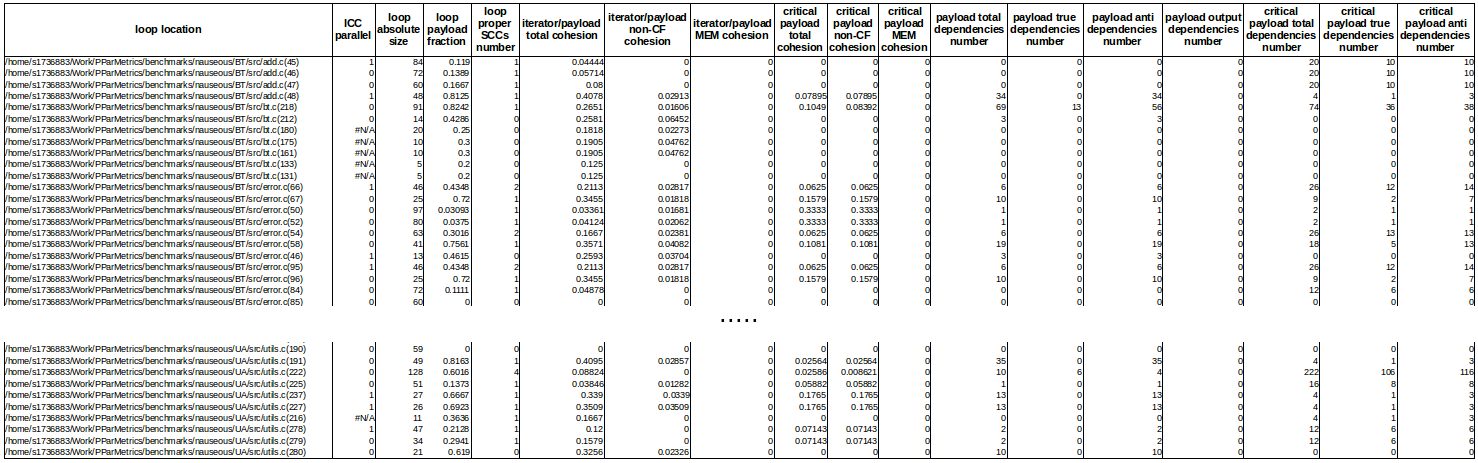
\includegraphics[width=\linewidth]{figs/metrics-table.png}
\caption{Analysis input table with computed metrics for all NAS Parallel benchmarks loops and ICC parallelizability classification labels.}
\label{analysis-data-table}
\end{sidewaysfigure}
\null\qquad This data is, essentially, a set of loops found in NAS benchmarks. For every single loop a vector of metrics (loop features) has been computed. All loops have passed through Intel C/C++ compiler parallelisability analyses and have been classified (labelled) as parallelizible or not. ICC compiler plays a role of an expert in this project. The table \ref{analysis-data-table} contains around 1400 loops with 13-dimensional feature vector for each.\newline
\null\qquad This dataset has been analysed in several ways. First, the collected data has been visualized to see if there are any obvious correlations between loop parallelisability property and metric values. Section \ref{analysis-data-interpretation-and-visualization} presents these visualizations and describes all found correlations. This visualization has been done for every single metric (see subsection \ref{analysis-single-metrics-vs-parallelizability}), as well as for the whole set of metrics altogether (see subsection \ref{analysis-data-clustering-analysis}). To visualize the whole combined set of metrics Principal Component Analysis (PCA) and clustering techniques have been used. A decision tree is another visualisation technique, that has been applied to the dataset (see subsection \ref{analysis-decision-tree}). Section \ref{analysis-manual-analysis} supplements these visualizations with some manually derived insights into benchmarks source code.\newline
\null\qquad As another mean of parallelizability metrics examination, statistical analysis techniques have been applied to the data. Loop metrics have been viewed as machine learning features in the context of loop parallelizability classification problem. Standard state-of-the-art  machine learning techniques (such as Support Vector Machines (SVM), desicion trees and neural network based Multi-layer Perceptron (MLP) scikit learn algorithm) have been applied to the data and all prediction errors have been compared against random predictor. Section \ref{analysis-statistical-analysis} presents a report on this.\newline
\null\qquad There has already been an attempt to apply statistical analysis techniques to see how software quality metrics, such as cyclomatic complexity \ref{background-cyclomatic-complexity} and Halstead's software science measures \ref{background-halsteads-measures} behave on Mozilla Firefox browser and LLVM compiler components library open source codes \cite{source-code-quality-classification-paper}. Authors applied k-means clustering and got 3 clusters of software quality metric values for subroutines. But there were no classifications attached to the input data and no correlations have been examined. There could easily be subroutines of different software quality grades in the same cluster. \newline
\null\qquad All results have been derived thanks to Python programming language and its packages: pandas \cite{python-lib-pandas}, matplotlib \cite{python-matplotlib} and scikit-learn \cite{python-lib-scikit-learn}. 

\section{Analyses preparation phase}
\label{analysis-preparation-phase}
\qquad Before we move onto the actual description of gathered results, there is a need to describe some preparatory data preprocessing procedures, which have been used throughout all analysis stages.\newline
\null\qquad As it turned out, there are some outliers in the collected data that distort the final result. For example, figure \ref{outliers-filtering} shows the plot of payload total dependencies number metric values on all NAS benchmark loops. The plot at the top shows metric values dispersion before outliers elimination. It can be seen that there is a non-parallelizible (red dot) loop with almost 12000 dependencies in the payload, which seriously shifts mean metric values for parallelizible and non-parallelizible subsets to the point of correlation inversion. Generally, it makes sense that the more dependencies we have in the payload, the harder it has to be to parallelize the loop. And it is seen from the whole dataset that loops with really high dependencies numbers have not been parallelized by the ICC compiler. But for majority of loops, encountered in NAS benchmarks, this tendency does not take place. 
\begin{figure}[H]
	\centering
	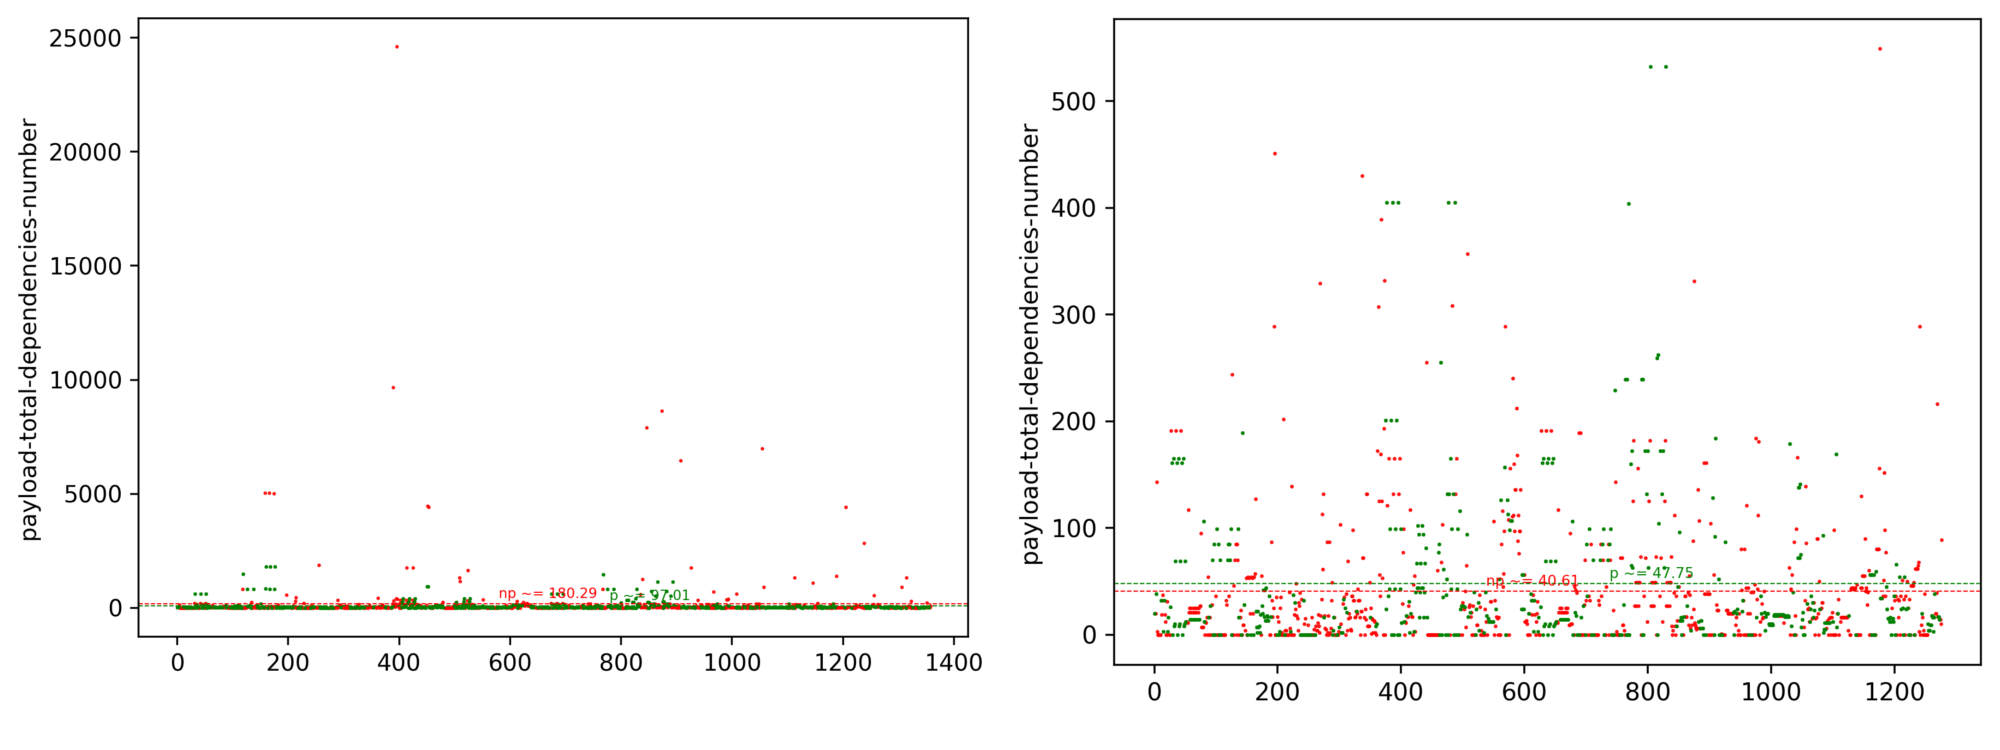
\includegraphics[width=\linewidth]{figs/outliers-filtering.png}
	\caption{Distribution of total dependencies number metric values on all NAS benchmark loops before and after elimination of all cases beyond 3 standard deviations from the mean.}
	\label{outliers-filtering}
\end{figure}  
\qquad The plot at the bottom contains only those loops, which have metric values withing 3 standard deviations from the mean. Here ICC parallelization ability does not really correlate with the amount of dependencies in the payload of the loop.\newline
\null\qquad The total number of dependencies in the payload of a loop is not the only metric, where we have some outliers. Similar filtering measures have been taken for all metrics. There was also a need to normalize the data before application of Principal Component Analysis (PCA) algorithm, in order to make a better graphical visualization.

\section{Data interpretation and visualization}
\label{analysis-data-interpretation-and-visualization}
\qquad This section presents different attempts to find any patterns and correlations in the data from the table \ref{analysis-data-table}. First, every single metric (out of all 13 presented in the table metrics) has been examined alone. Section \ref{analysis-single-metrics-vs-parallelizability} contains all results of single metric parallelizability analysis. Then, the set of metrics has been considered altogether as a whole (as points in 13-dimensional space) in order to find any structural patterns they form. Principal Component Analysis and k-means clustering have been used for that task. Results are presented in subsection \ref{analysis-data-clustering-analysis}. And then, finally, decision trees have been used to derive parallelizability classifications out of the data and visualize that derivation (see subsection \ref{analysis-decision-tree}). 
\subsection{Single loop metrics vs loop parallelisability analysis}
\label{analysis-single-metrics-vs-parallelizability}
\qquad The layout of this section corresponds to that of section \ref{metrics-metric-groups}, which describes proposed groups of software parallelizability metrics. Subsections below present studies of their parallelizability correlation.
\subsubsection{Loop proportion metrics}
\label{analysis-loop-proportion-metrics}
\qquad Figures \ref{loop-proportions-0} and \ref{loop-proportions-1} present scattered plots of all loop proportion metric values, gathered on NAS benchmark loops. Numbers on vertical axes represent metric values, values on horizontal axes represent particular loops in the set. Dashed horizontal lines, crossing plots, represent mean values for subsets of parallelizible (green) and non-parallelizible (red) loops. Numbers show how many dots lie above and below mean values for red and green subsets. All outliers lying beyond 3 standard deviations have been filtered (see section \ref{analysis-preparation-phase}).
\begin{figure}[H]
\centering
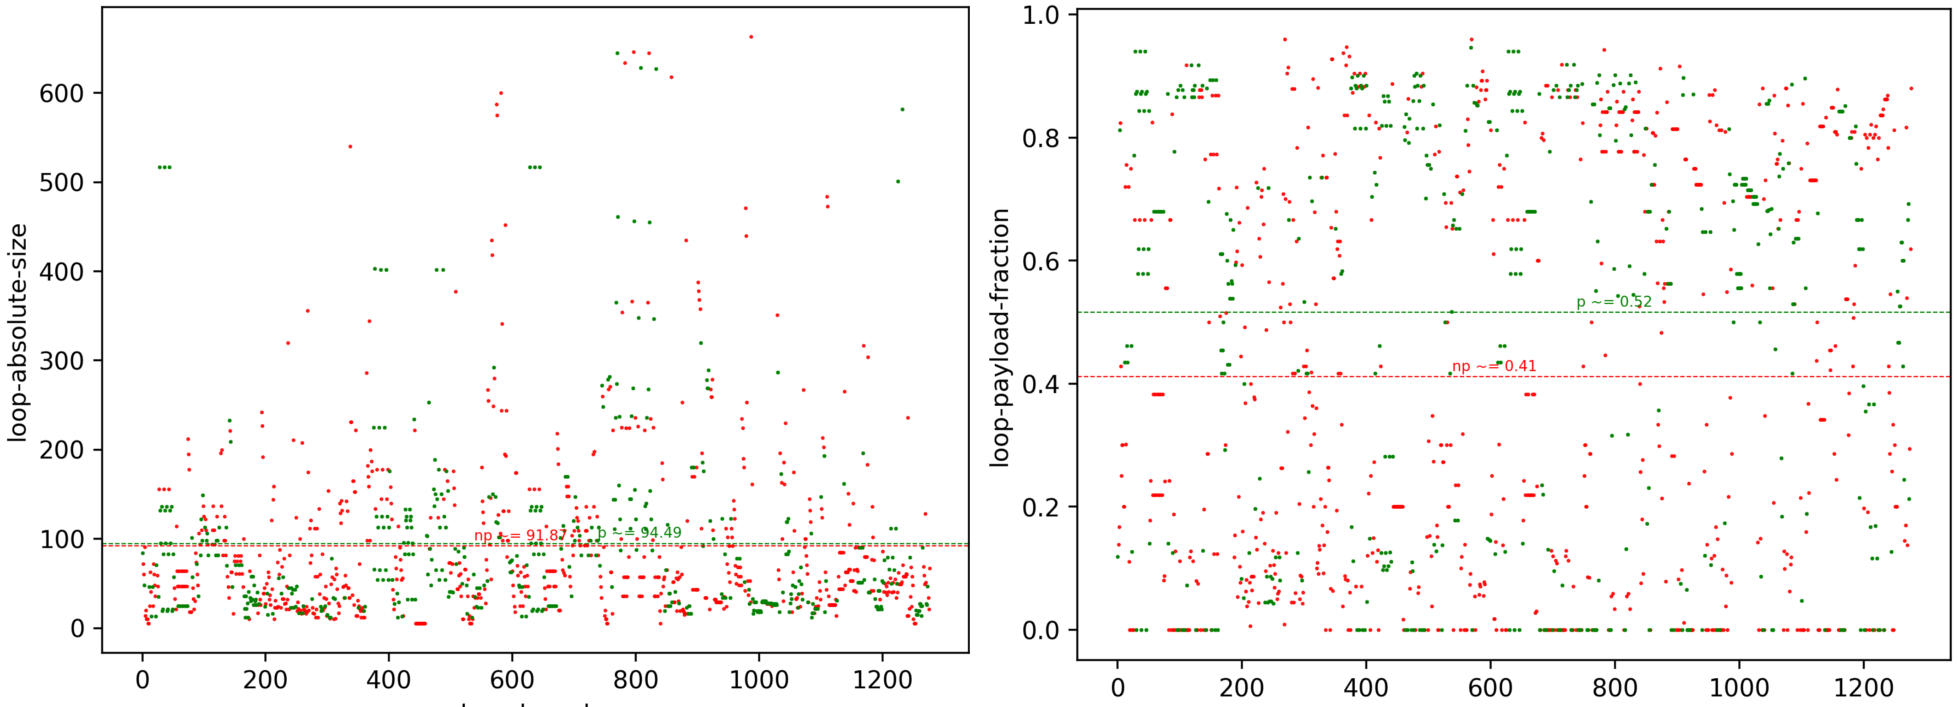
\includegraphics[width=\linewidth]{figs/loop-proportions-0.png}
\caption{\textit{Loop absolute size} metric at the top and \textit{loop payload fraction} metric at the bottom. Red and green dots represent loops, which have not/have been parallelized by ICC compiler correspondingly. Dashed lines show mean metric values for red and green subsets correspondingly.}
\label{loop-proportions-0}
\end{figure}
\begin{figure}[H]
\centering
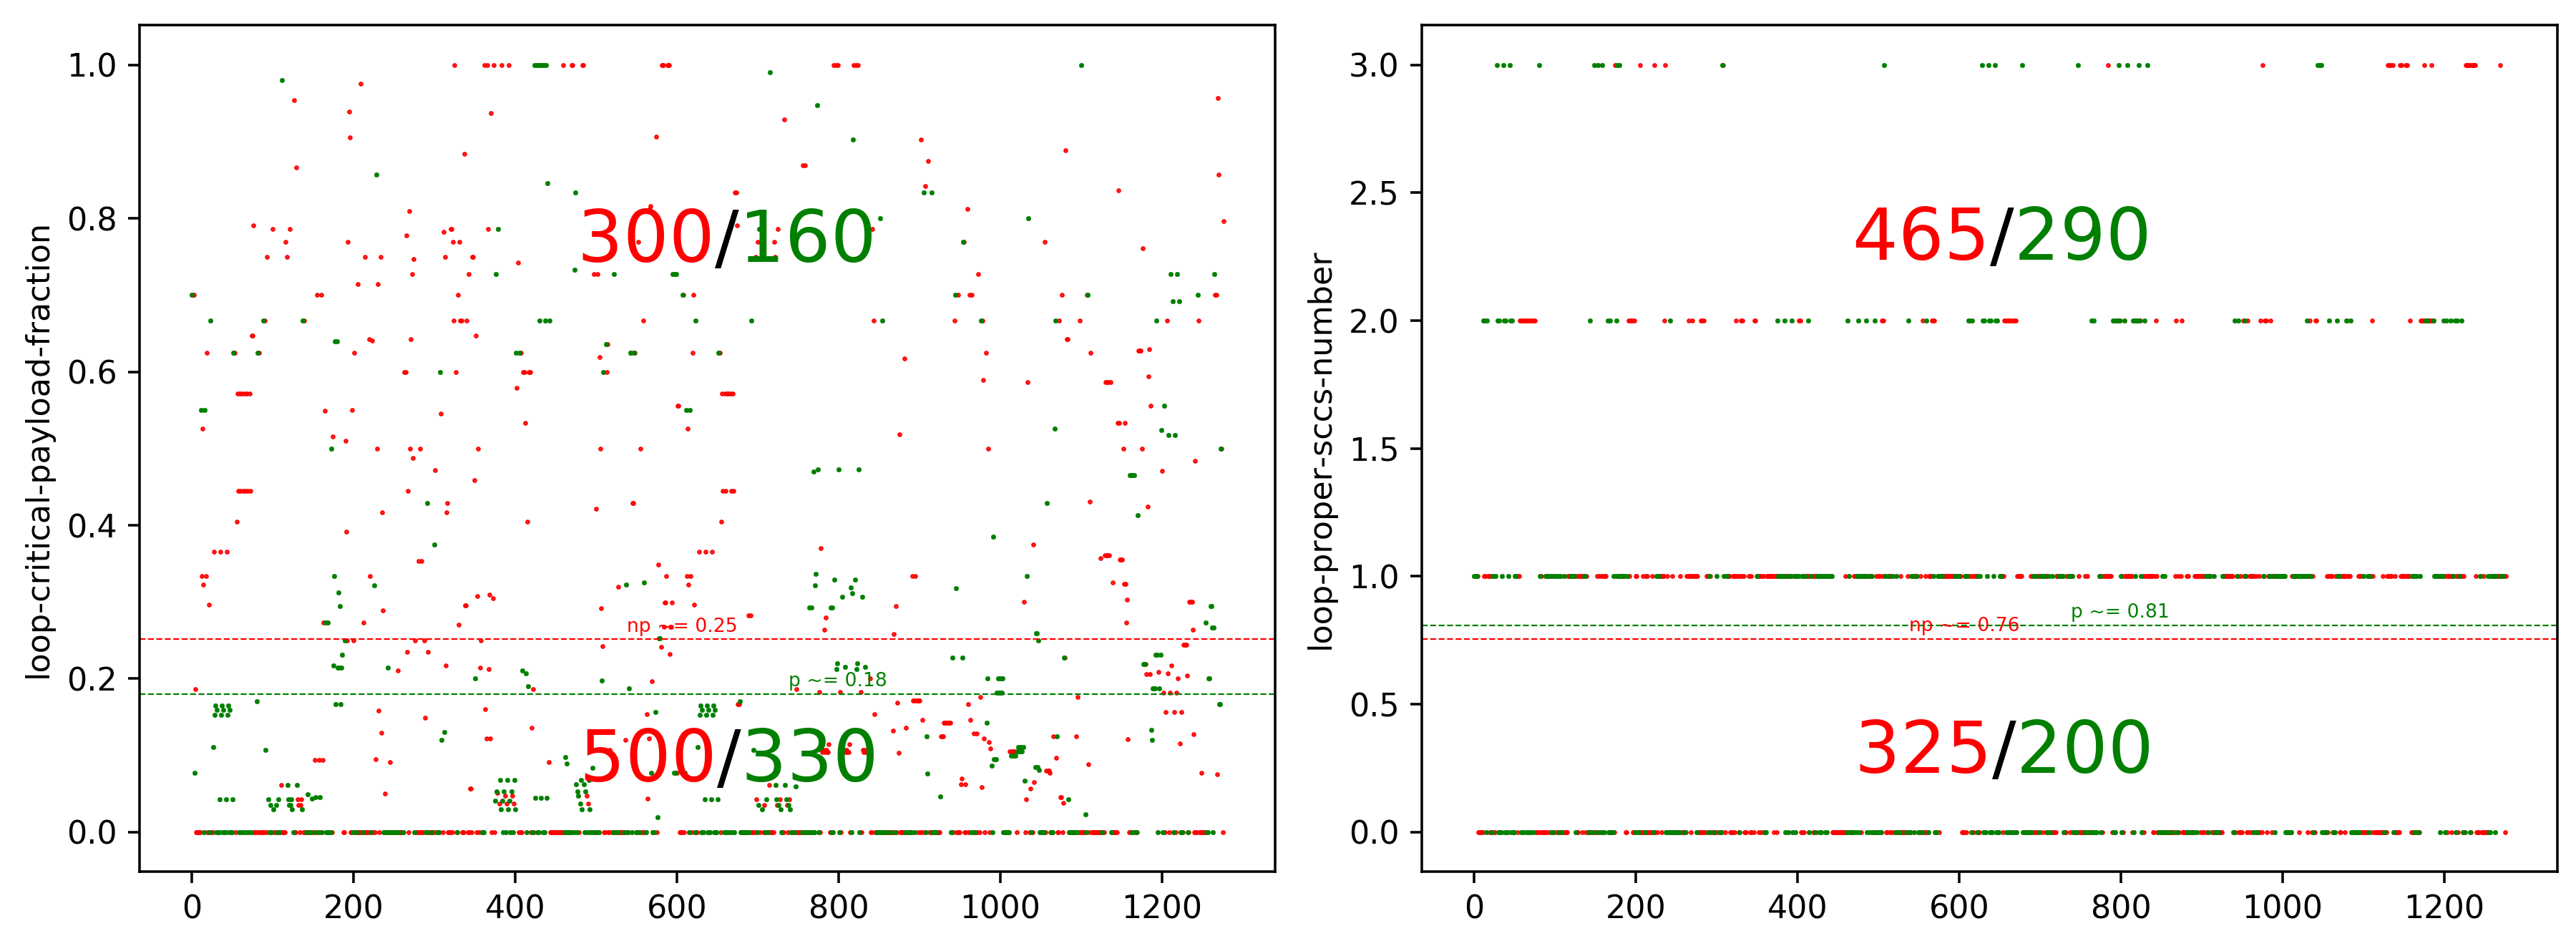
\includegraphics[width=\linewidth]{figs/loop-proportions-1.png}
\caption{\textit{Loop critical payload fraction} metric at the top and \textit{loop proper SCCs number} metric at the bottom. Analogous to \ref{loop-proportions-0} figure.}
\label{loop-proportions-1}
\end{figure} 
\quad As it can be seen from the plots, \textit{loop absolute size} metric values do not correlate with ICC parallelization ability. Mean values of that metric are almost identical, ~91,87 and 94,49 LLVM-IR instructions, for non-parallelizible and parallelizible loop subsets correspondingly. Red and green dots are scattered above and below mean value lines in similar proportions (210/580$\approx$0,36 and 120/360$\approx$0,33) - majority of NAS loops are smaller than 90 LLVM-IR instructions.\newline
\null\qquad It must be clear from the nature of this metric, that size by itself does not prohibit loop parallelization. There might be a big loop with no cross-iteration dependencies, which must have a big portion of parallelism and should bring huge overall performance gains with its parallelization. And vice versa, there might be a small loop with cross-iteration dependency, which is non-parallelizible.\newline
\null\qquad There is a noticeable correlation between loop parallelisability and values of \textit{loop payload fraction} metric. Green dots are scattered predominantly at the top of the plot. Dot numbers above and below mean lines are in inverse proportionality for red and greed dot subsets (370/420$\approx$0,88\textless 1 and 300/190$\approx$1,58\textgreater 1).  The bigger the payload of a loop in comparison with its iterator, the more seducing this loop for compiler to parallelize. Bigger payloads bring better performance gains with parallelization. Another consideration might also be applied here. Bigger iterators are common for loops, which, for example, perform traversal of more complex data structures like linked-lists or alike. Such loops contain memory operations linking iterator and payload - \textit{iterator payload memory cohesion} metric should be non zero for such loops. Unfortunately, there are no such loops in NAS benchmark set and the latter metric has been excluded from consideration at all.\newline 
\null\qquad Despite the fact that \textit{loop proper SCCs number} metric does not correlate with loop parallelizability that much, another metric of the same essense shows pretty good correlations. \textit{Loop critical payload fraction} metric can be used to judge about loop parallelizability. Connection between this metric and parallelizability property follows just out of the common sense. Critical payload parts represent strongly connected components with more than one instructions. There are PDG graph loops with forward and back edges inside such SCCs. Usually it happens when two memory instructions reference the same location on different (or the same) loop iterations and introduce 2 inverse-directed edges with anti and true dependencies. Such critical loop payload parts introduce actual parallelization constraints. The left plot in the figure \ref{loop-proportions-1} illustrates this connection. The bigger the critical component in the payload, the harder it is to parallelize the loop.
\begin{figure}[H]
	\centering
	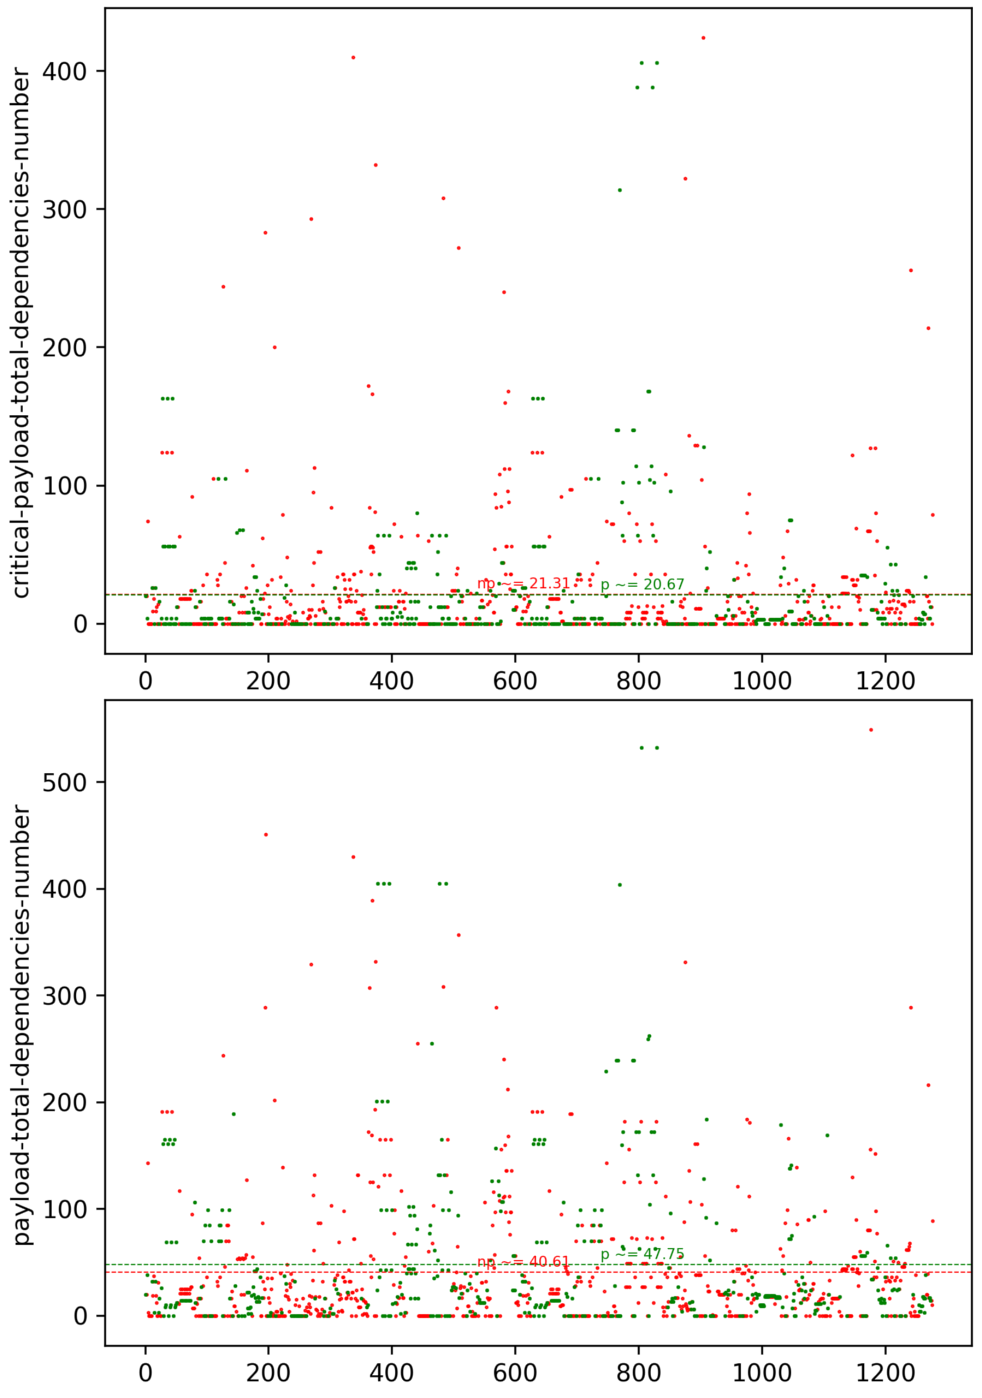
\includegraphics[width=\linewidth]{figs/loop-dependencies-number-0.png}
	\caption{\textit{Critical payload dependencies number} metric at the top and \textit{total payload dependencies number} metric at the bottom. Red and green dots represent loops, which have not/have been parallelized by ICC compiler correspondingly. The other 4 metrics show similar behavior and have been moved into appendix section (see plots \ref{loop-dependencies-number-1} and \ref{loop-dependencies-number-2}).}
	\label{loop-dependencies-number-0}
\end{figure}
\subsubsection{Loop Dependence Metrics}
\label{analysis-loop-dependence-metrics}
\qquad Figures \ref{loop-dependencies-number-0}, \ref{loop-dependencies-number-1} and \ref{loop-dependencies-number-2} present plots of loop dependencies number metric values. These metrics do not seem to be particularly reliable, when it comes to judging about loop parallelizability. Due to this reason the two latter plots have been moved into appendix section.\newline
\null\qquad As it can be seen from the figures, distributions of parallelizible and non-parallelizible (green and red) dots are quite uniform throughout the whole spectrum of metric values. Mean metric values on green and red subsets are also close to each other. In cases, where they differ, that difference dissappears with addition of excluded outliers to consideration. Even for loops with a huge total dependencies number either in critical part or in the whole loop payload, ICC compiler sometimes is able to generate a parallel version. All these points show that loop dependencies number metrics cannot be used alone for loop parallelizability analysis.

\subsubsection{Loop Cohesion Metrics}
\label{analysis-loop-cohesion-metrics}
\qquad Loop cohesion metrics have been described in section \ref{metrics-loop-cohesion-metrics}. Figures \ref{loop-cohesion-0} and \ref{loop-cohesion-1} present plots of loop cohesion metric values on the set of NAS benchmark loops (roughly 1300 loops).\newline
\qquad Critical payload cohesion metrics do not correlate that much with parallelizability property. Figure \ref{loop-cohesion-0} shows approximately similar mean metric values on red and green subsets and it is also visible, that red and green dots are uniformly dispersed on the plane. These cohesion metrics represent the degree of interconnection between critical part of loop payload and its non-critical part.\newline
\null\qquad On the other hand, \textit{iterator payload cohesion} metrics show a certain degree of correlation with loop parallelizability. It is visible from the two plots on figure \ref{loop-cohesion-1}, that green parallelizible dots are dispersed predominantly at the top of the plane. Mean metric values on red and green subsets tell exactly the same thing: mean metric values for parallelilazible loops tend to be higher than their counterparts on non-parallelizible subsets (0,25 versus 0,20 for \textit{iterator payload total cohesion} and 0,03 versus 0,02 for \textit{iterator payload non-cf cohesion}). Dot numbers above and below mean lines are also in inverse proportionality, as it is visible from figure \ref{loop-cohesion-1}.   
\begin{figure}[H]
\centering
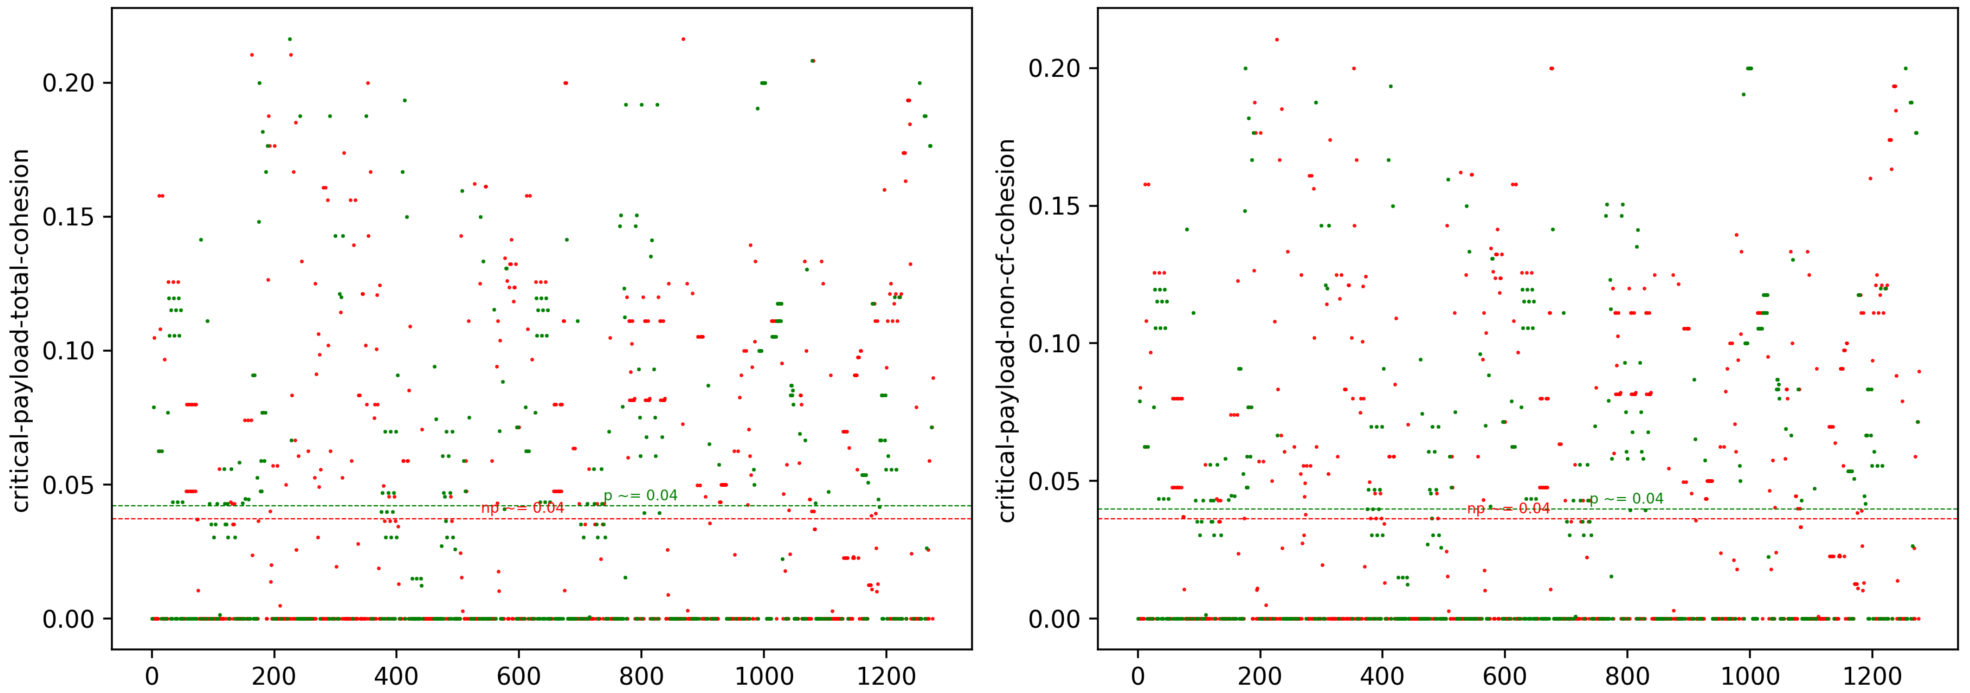
\includegraphics[width=\linewidth]{figs/loop-cohesion-0.png}
\caption{\textit{Critical payload total cohesion} metric at the top and \textit{critical payload non-cf cohesion} metric at the bottom. Red and green dots represent loops, which have not/have been parallelized by ICC compiler correspondingly.}
\label{loop-cohesion-0}
\end{figure}
\begin{figure}[H]
\centering
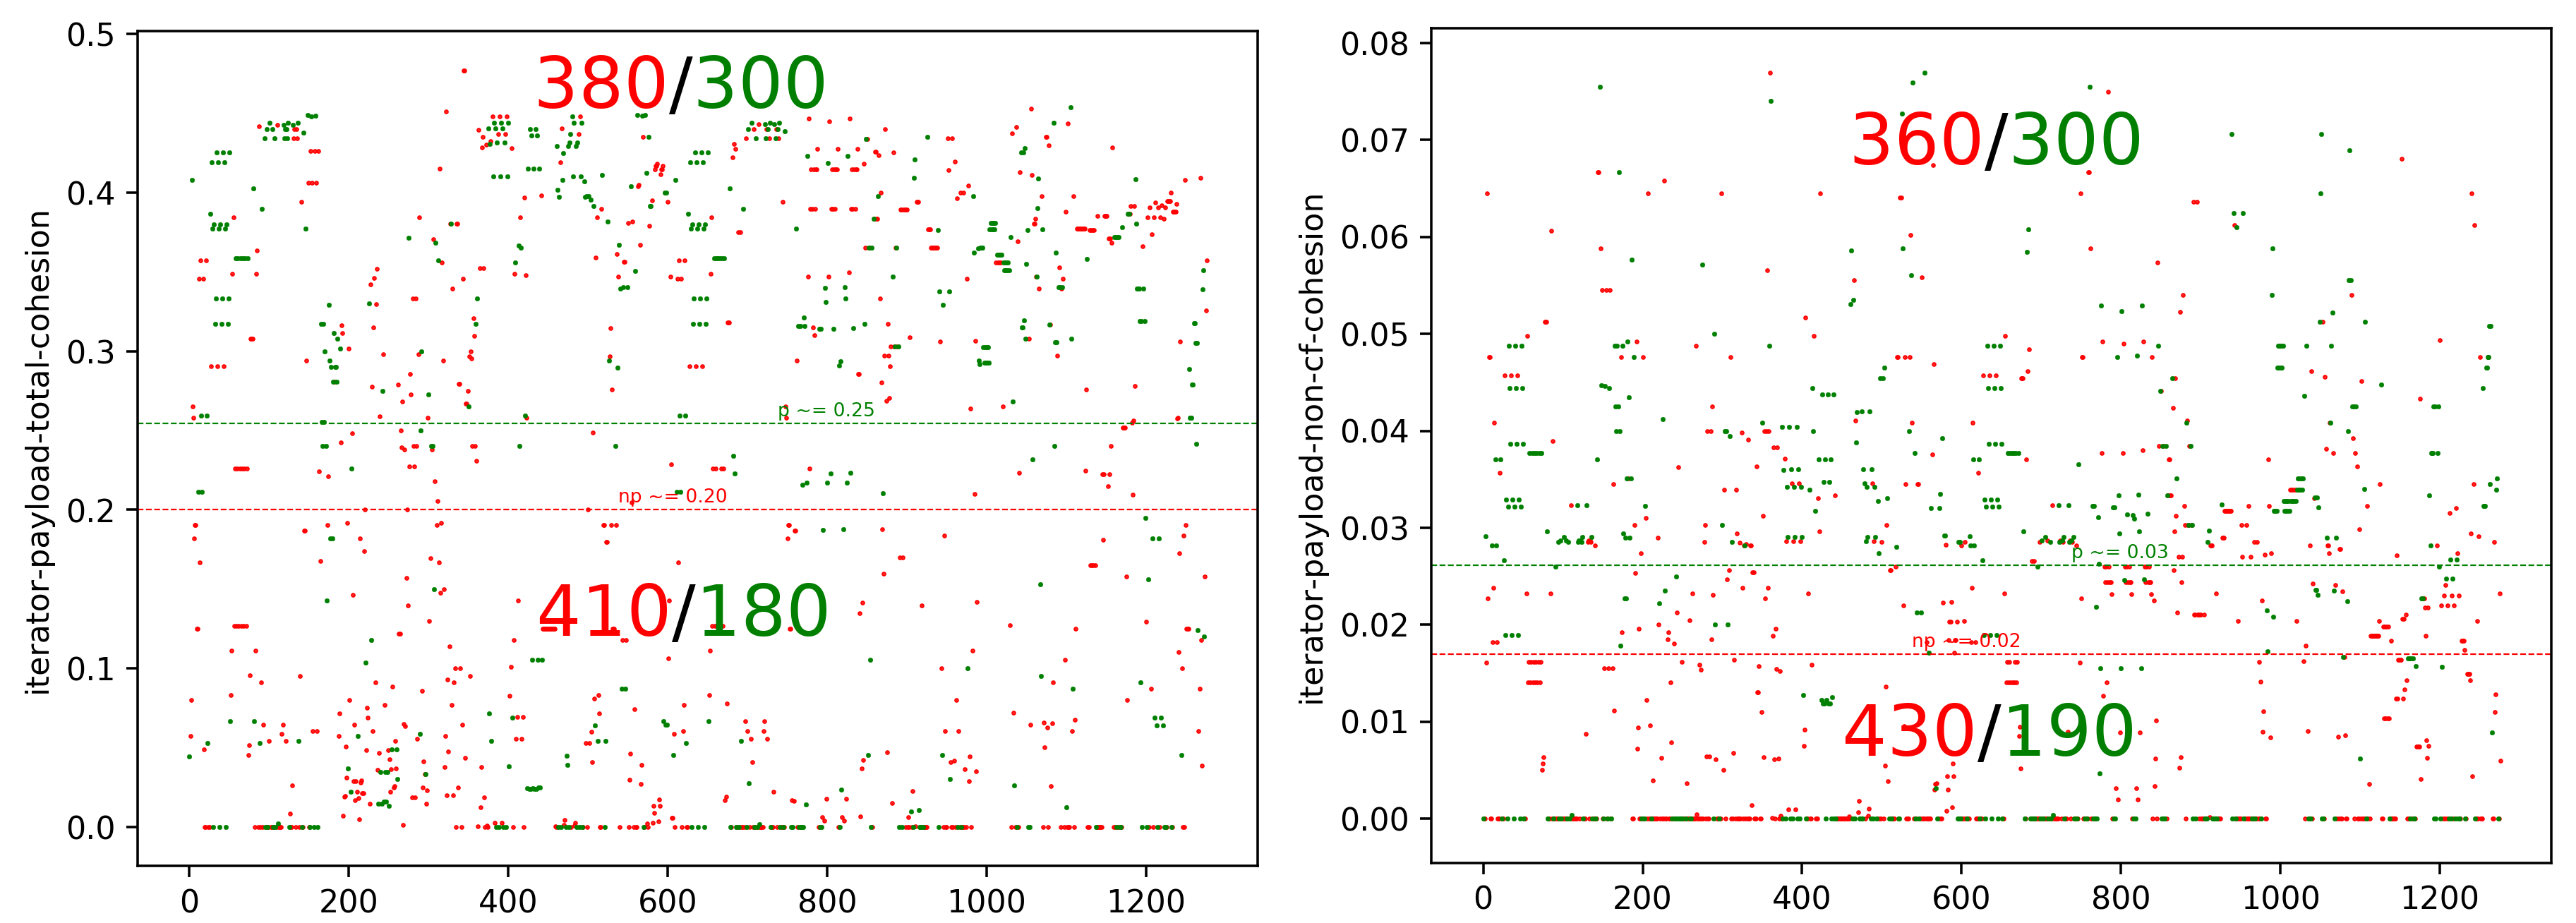
\includegraphics[width=\linewidth]{figs/loop-cohesion-1.png}
\caption{\textit{Iterator payload total cohesion} metric at the top and \textit{Iterator payload non-cf cohesion} metric at the bottom. Red and green dots represent loops, which have not/have been parallelized by ICC compiler correspondingly.}
\label{loop-cohesion-1}
\end{figure}
 
\subsection{Data clustering analysis}
\label{analysis-data-clustering-analysis}
\qquad This section describes the results of dataset clustering analysis. Data from the table \ref{analysis-data-table} can be viewed as a set of 13-dimensional vectors, describing NAS benchmark loops. These vectors map loops into 13-dimensional space. It might be interesting to see what spatial patterns and structural properties these mappings conform to. For every loop, thanks to Intel C/C++ compiler, we know the right answer regarding its parallelizability. This section reports studies about correlations between spatial and structural properties of these vector mappings and loops parallelizability.\newline
\begin{figure}[H]
\centering
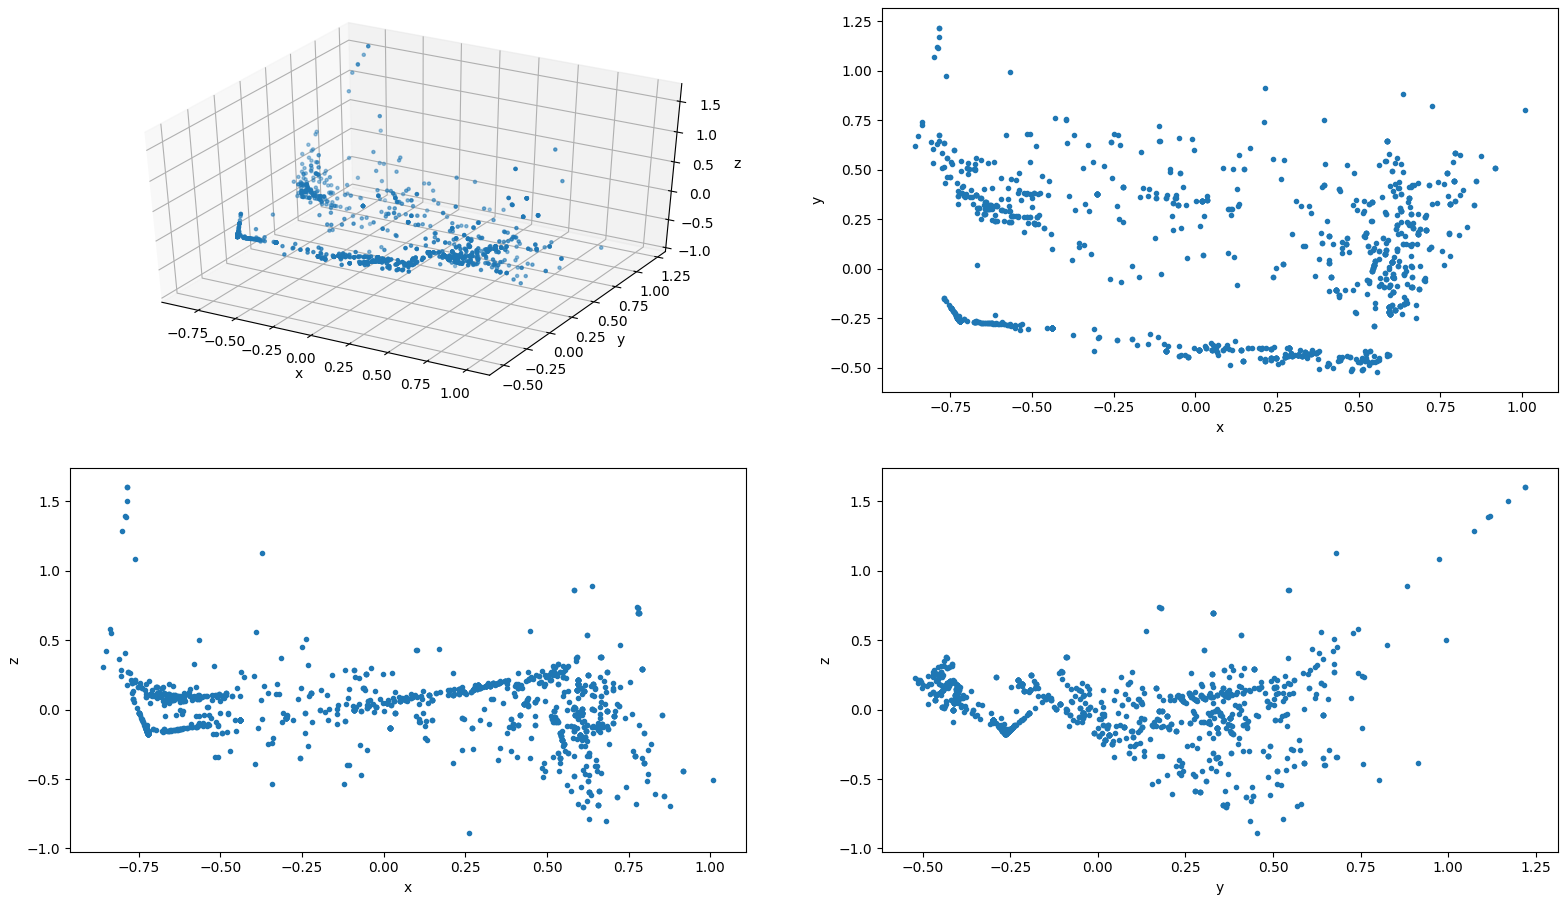
\includegraphics[width=\linewidth]{figs/metrics-pca-13-to-3.png}
\caption{Visualisation of loop metrics dataset spatial distribution (13-dimensional metric vectors have been projected onto 3D space thanks to PCA algorithm) - blue dots correspond to metric values of single loops.}
\label{metrics-pca-13-to-3}
\end{figure} 
\null\qquad Since loops are represented by 13-dimensional vectors, direct dataset visualization is unfeasible. Principal Components Analysis (PCA) has been used to project the data onto 3-dimensional space and visualize it. Figure \ref{metrics-pca-13-to-3} provides an illustration of distribution of metric values on all loops. It is visible from the figure, that data values do not form any apparent clusters, but there are some areas of increased density though. Metric dataset projection onto 2D plane looks like XY projection of 3D PCA mapping (see figure \ref{metrics-pca-13-to-2}).\newline
\null\qquad Next step is to establish correlation between structural properties of dataset distribution and loop parallelizability. Figure \ref{metrics-pca-parallelizability} provides an illustration for it. Out of that figure it is visible that there is no apparent correlation between combined metric values and parallelizability of loops these metrics represent. 
\begin{figure}[H]
\centering
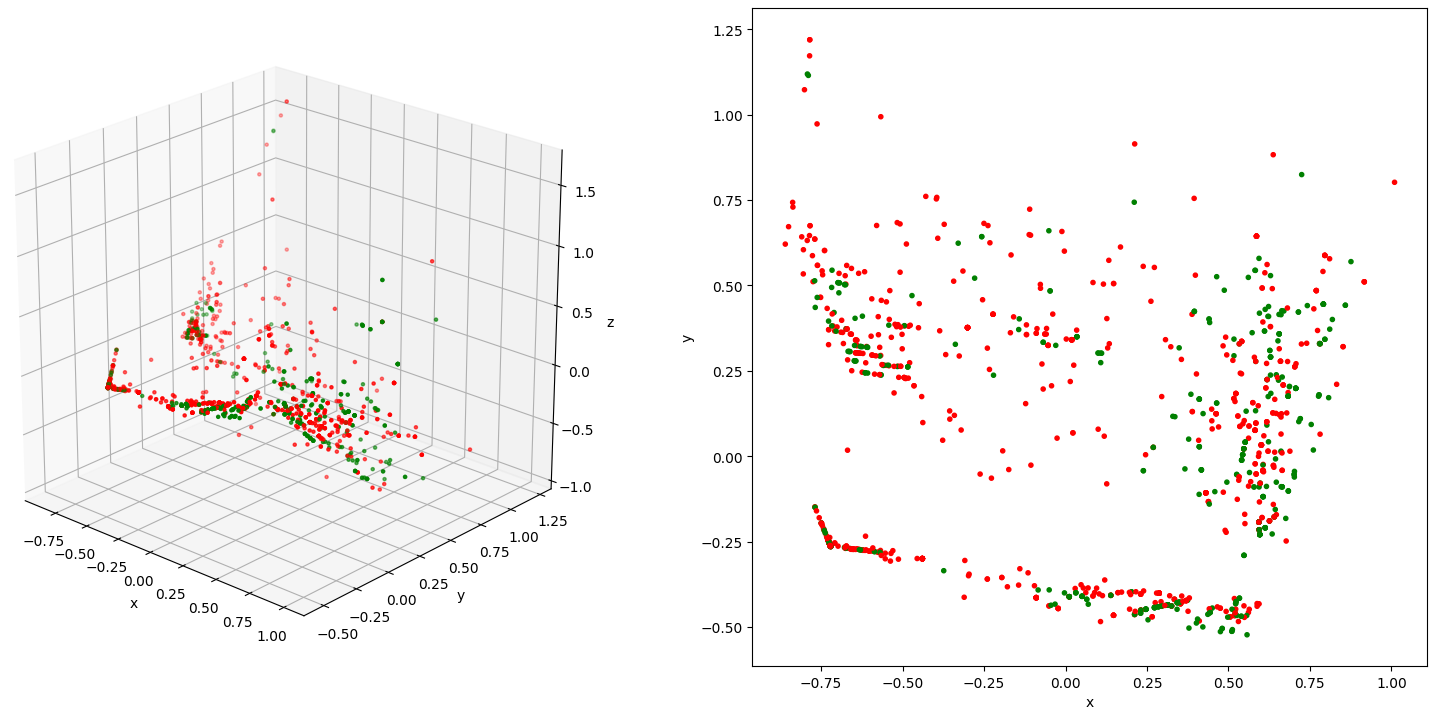
\includegraphics[width=\linewidth]{figs/metrics-pca-parallelizability.png}
\caption{Visualisation of loop metrics dataset spatial distribution (3D PCA projection on the left, 2D PCA projection on the right) versus parallelizability property. Red dots - non-parallelizible loops; green dots - parallelizible loops}
\label{metrics-pca-parallelizability}
\end{figure} 
\null\qquad It would be interesting to see, what kind of loops and metric values form these areas of increased density. To get that information we can apply k-means clustering algorithm and get subsets of loops, which form these condensed clots. We need to pick the number of clusters. The number of clusters might be arbitrary, but from the figure it is visible that 3 or 4 clusters would be quite a close approximation to the given dots distribution. Figure \ref{metrics-4-clusters} illustrates the results of k-means clustering algorithm run with 4 clusters. Algorithm has almost perfectly identified the structure of dots distribution. Maybe yellow and blue subsets must be in the same subset. We can consider all these blue and yellow loops altogether. Some dots (the ones on the boundary of red cluster) also happened to be blue, while red classification would be the most appropriate for them. To exclude these must-be-red blue loops from considerations applied to the blue cluster, euclidean distances from cluster centers were computed for every dot. Only loops near cluster centers are considered in the manual source code study. Table \ref{clusters-metric-values} presents average values for all metrics in 4 clusters. \newline
\begin{figure}[H]
\centering
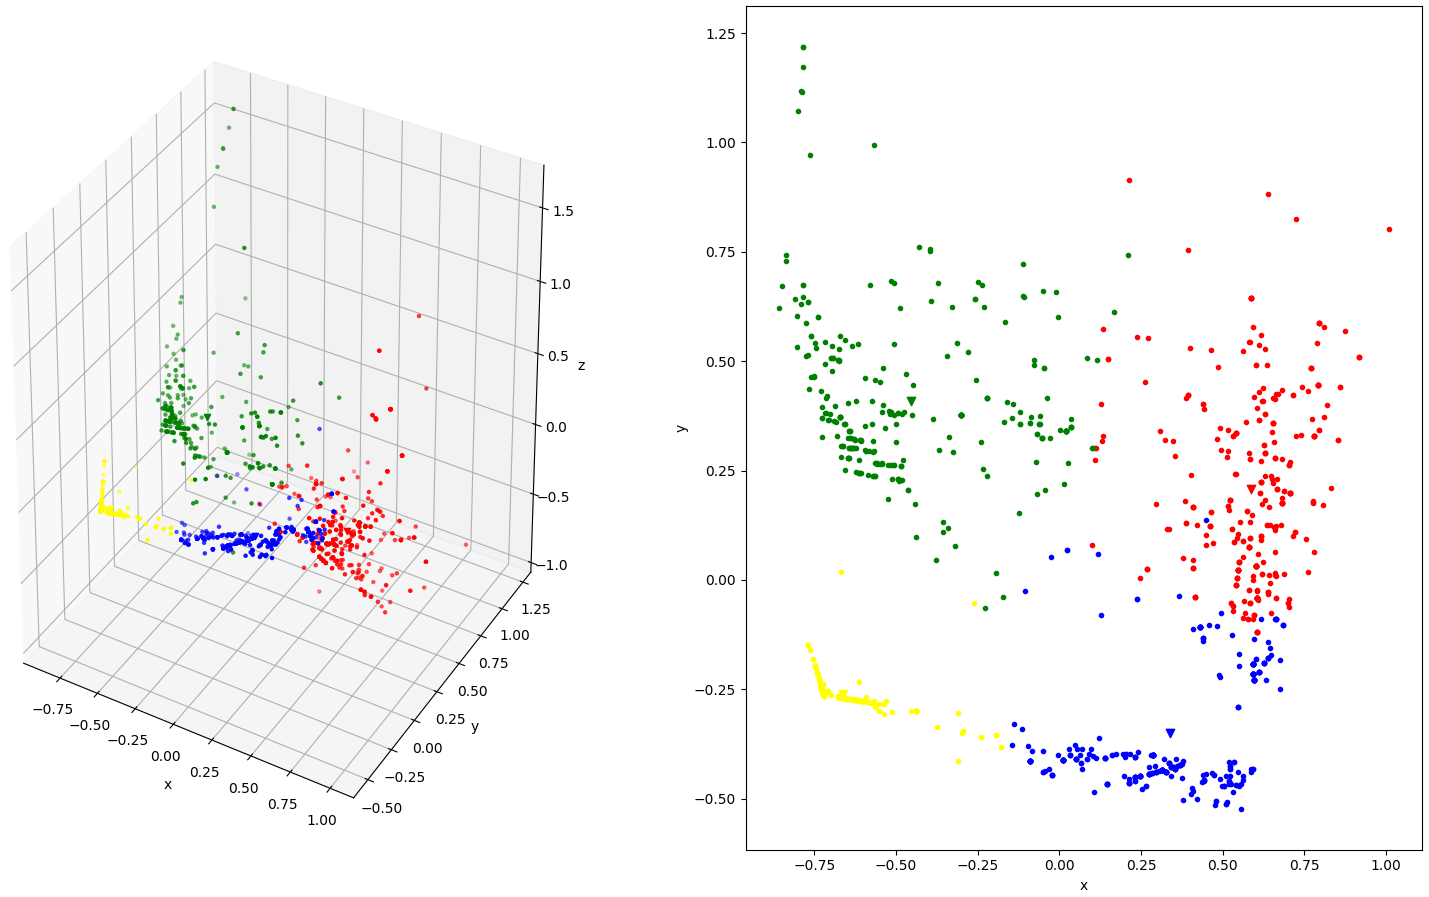
\includegraphics[width=\linewidth]{figs/metrics-4-clusters.png}
\caption{k-means algorithm classified the dataset into 4 separate clusters.}
\label{metrics-4-clusters}
\end{figure}
\begin{figure}[H]
\centering
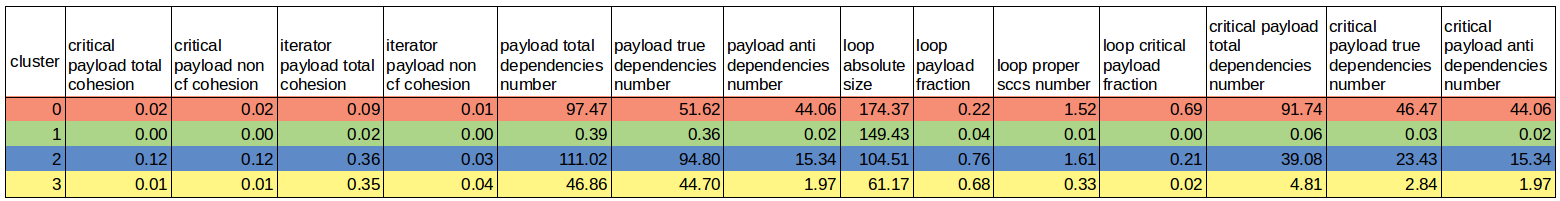
\includegraphics[width=\linewidth]{figs/clusters-metric-values.png}
\caption{Average metric values for 4 different clusters}
\label{clusters-metric-values}
\end{figure} 
\null\qquad Out of that table \ref{clusters-metric-values} and figure \ref{metrics-4-clusters} we can derive metric growth directions. All critical payload part related metrics show tendency to grow anti-clockwise, having minimum values in the green dot cluster and maximum values in the red one. We can combine all these metrics in one \textit{critical component size} characteristic. Cohesion between loop iterator and payload parts grows from green cluster towards all 3 other clusters, reaching its maximum values in blue and yellow clusters. \textit{Loop absolute size} has a mirrored (in relation to \textit{iterator payload cohesion} metric) pattern of growth. It starts to grow in the yellow cluster and takes on higher values as it reaches 3 other clusters. Figure \ref{clusters-metric-values} presents the final illustration for all considerations above.\newline   
\begin{figure}[H]
\centering
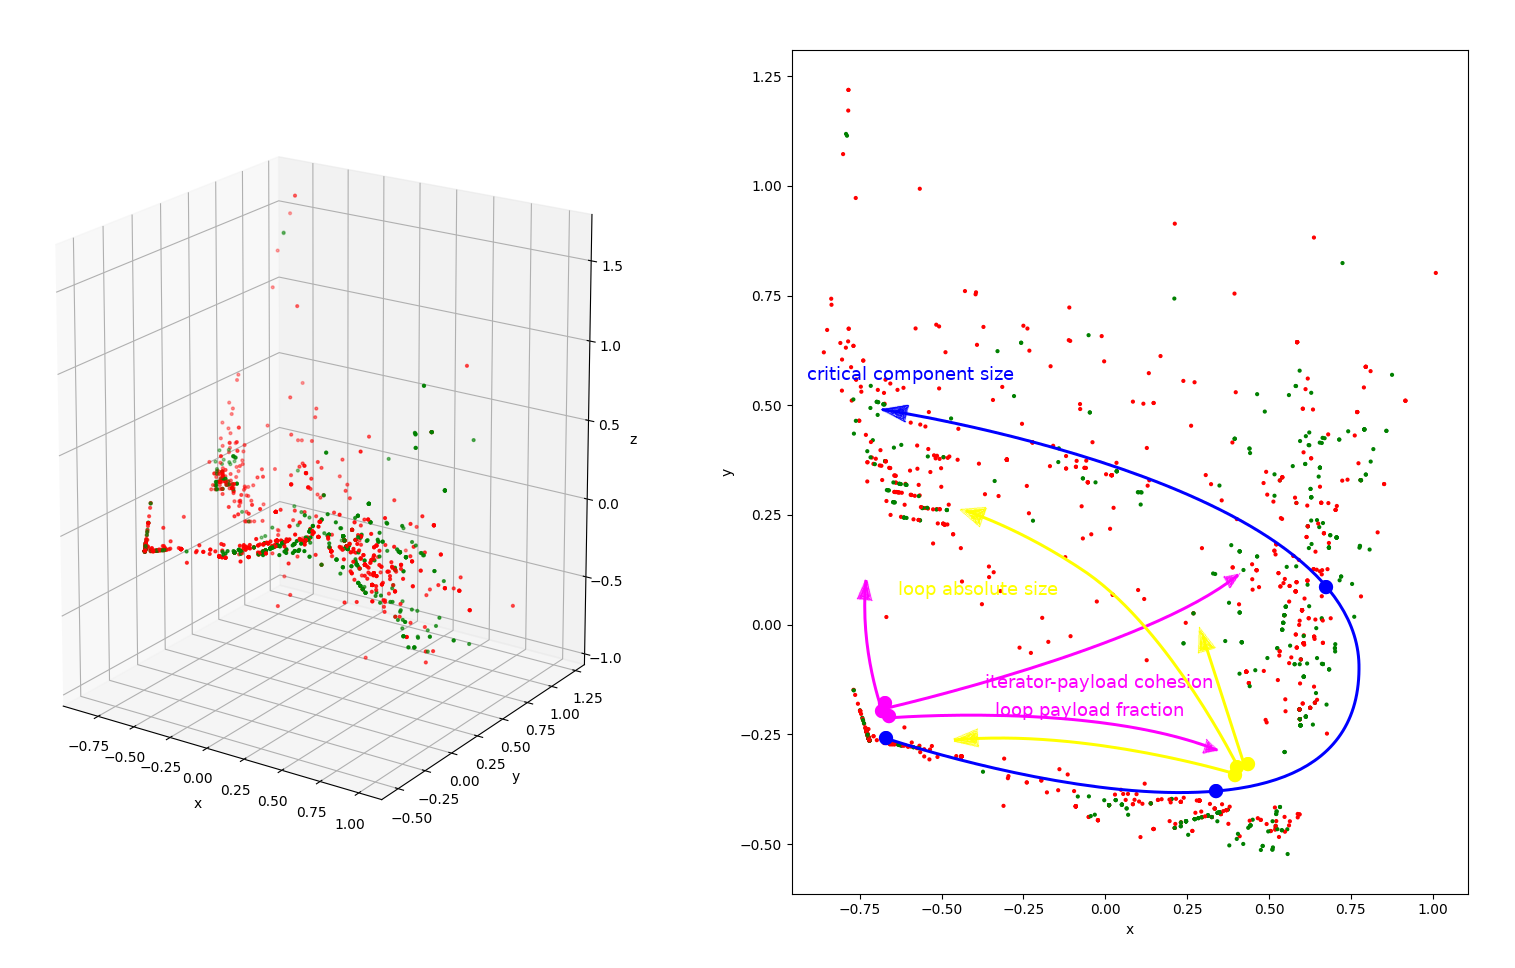
\includegraphics[width=\linewidth]{figs/metrics-growth-directions.png}
\caption{Correspondence between 3D PCA projected distribution and original metric values, set by growth arrowed lines.}
\label{clusters-metric-values}
\end{figure}
\null\qquad The next section \ref{analysis-manual-analysis} provides examples of loops, which can be found in these 4 built clusters.  

\subsection{Decision tree based parallelisability classification}
\label{analysis-decision-tree}
\qquad Decision tree is another human-comprehensible dataset visualization technique. Figure \ref{decision-tree-depth-3} has been produced with scikit-learn \cite{python-lib-scikit-learn} decision tree classifier and represents a decision tree learned from metrics table dataset \ref{analysis-data-table}. Decision tree sorts metric vectors down the tree. Sorting starts from the root and goes along all the sorting rules down to the leaf. Leaf provides the final metric vector classification. For simplicity and feasibility of visualisation, the depth of the tree has been limited to 3. This limitation leads to some probabilistic errors in the final loop parallelizability classification, but is still capable of capturing the main trends in the data. \ref{analysis-data-table}.\newline
\null\qquad The construction of decision tree is based on the notions of entropy and information gain. Decision tree algorithm finds and places in the root of the tree a rule, which separates the dataset in a way, that brings the biggest information gain (in other words, decreases entropy of the dataset the most). Then it goes along all the branches down the tree and places the most information gaining rule at every node, calculated on the dataset subset, corresponding to that node.\newline
\null\qquad As we can see from the figure \ref{decision-tree-depth-3}, scikit-learn implementation of decision tree algorithm picked \textit{iterator-payload non-cf cohesion} as a metric, separating the input dataset in the best way. The input dataset contains 1277 metric vectors, 790 of them are classified as non-parallelizible and 487 as parallelizible. The entropy of such a dataset equals to $S=-\frac{790}{1277}\cdot \log_{2}\frac{790}{1277}-\frac{487}{1277}\cdot \log_{2}\frac{487}{1277}\approx 0.96$. After the rule in the root split the dataset into two subsets, corresponding to the left and right subtrees, the entropy became $S=\frac{790}{1277}\cdot S_{True} + \frac{487}{1277}\cdot S_{False} = \frac{793}{1277}\cdot (-\frac{591}{793}\cdot \log_{2}\frac{591}{793}-\frac{202}{793}\cdot \log_{2}\frac{202}{793}) + \frac{484}{1277}\cdot (-\frac{199}{484}\cdot \log_{2}\frac{199}{484}-\frac{285}{484}\cdot \log_{2}\frac{285}{484})\approx 0.8787 $. And so on.\newline
\begin{sidewaysfigure}
	\centering
	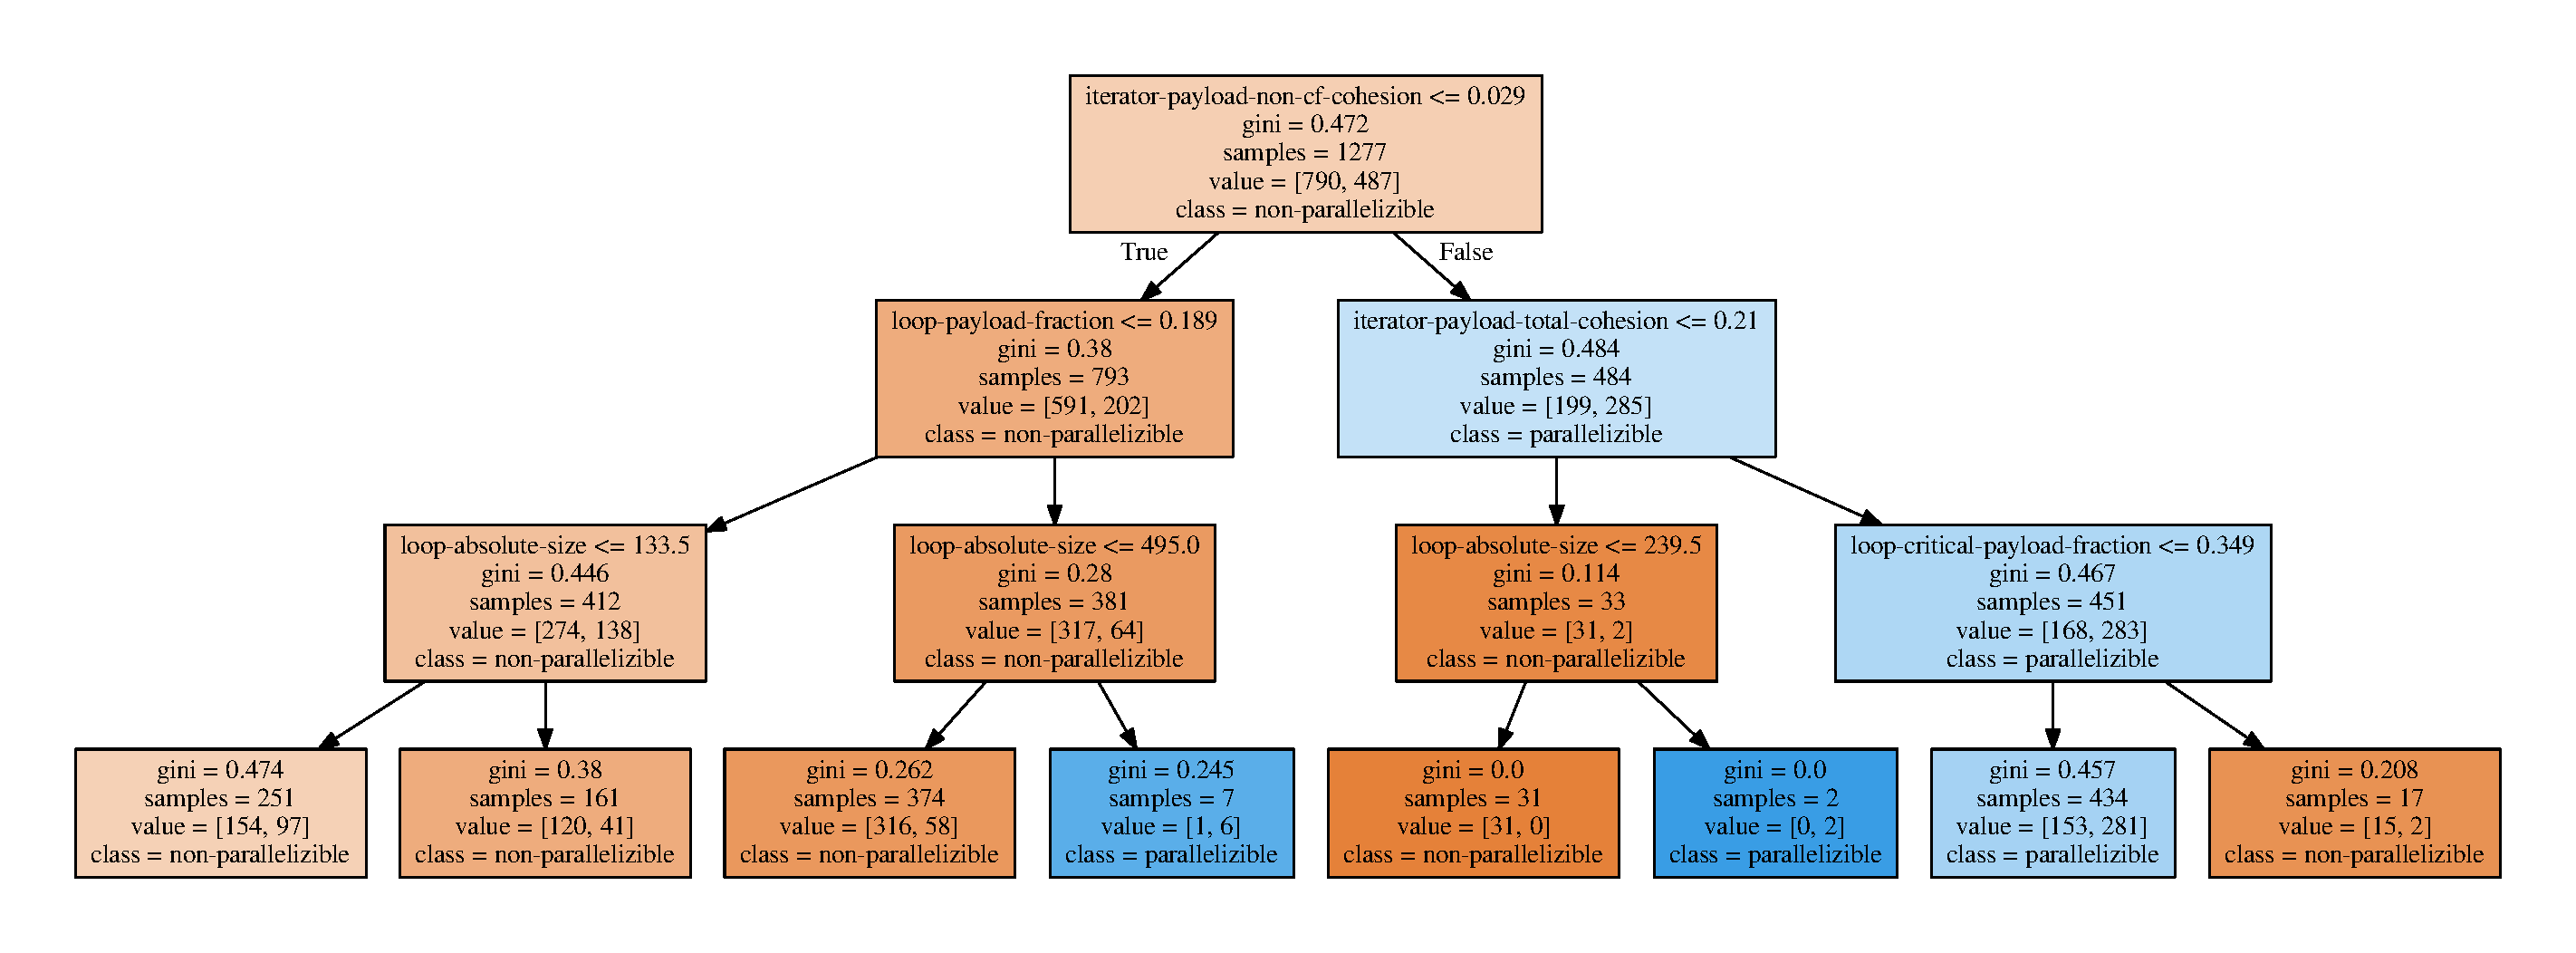
\includegraphics[width=\linewidth]{figs/decision-tree-depth-3.pdf}
	\caption{Dataset \ref{analysis-data-table} decision tree, limited to the depth of 3.}
	\label{decision-tree-depth-3}
\end{sidewaysfigure}
\null\qquad For the purpose of our work we can interpret that decision tree in the following way. If we use \textit{iterator-payload non-cf cohesion} metric to judge about loop parallelizability, then we should compare the value of that metric for a loop being considered against 0,03. If the value on the loop is greater than 0,03, then the loop is parallelizible with probability of $\frac{285}{484}\approx 60\%$ and non-parallelizible with probability of $\frac{199}{484}\approx 40\%$. That numbers do not give us a lot of information, but if value of the metric on a loop happens to be below 0,03, then the loop is most likely to be non-parallelizible with probability of $\frac{591}{793}\approx 75\%$. The latter signals loop code developer to reconsider his code, if he wants his code to take advantage of parallelization.\newline
\null\qquad These are basically the same results as ones in the section \ref{analysis-single-metrics-vs-parallelizability} of the current chapter, but decision tree methods have more solid mathematical grounds and foundation. Decision tree algorithm automatically finds a decision boundary in the range of single metric values, that splits the dataset in the most information gaining way. The tree on the figure \ref{decision-tree-depth-3} has been built from the set of all 13 metrics. According to the algorithm criteria \textit{iterator-payload non-cf cohesion} metric is the best for loop parallelizability analysis task. If we exclude that metric from the set of metrics for the root rule search, or even use just one metric, we can find decision boundaries with corresponding probabilities for all more or less parallelizability correlating metrics. Figure \ref{decision-trees-single-metrics} shows the result.
\begin{figure}[H]
\centering
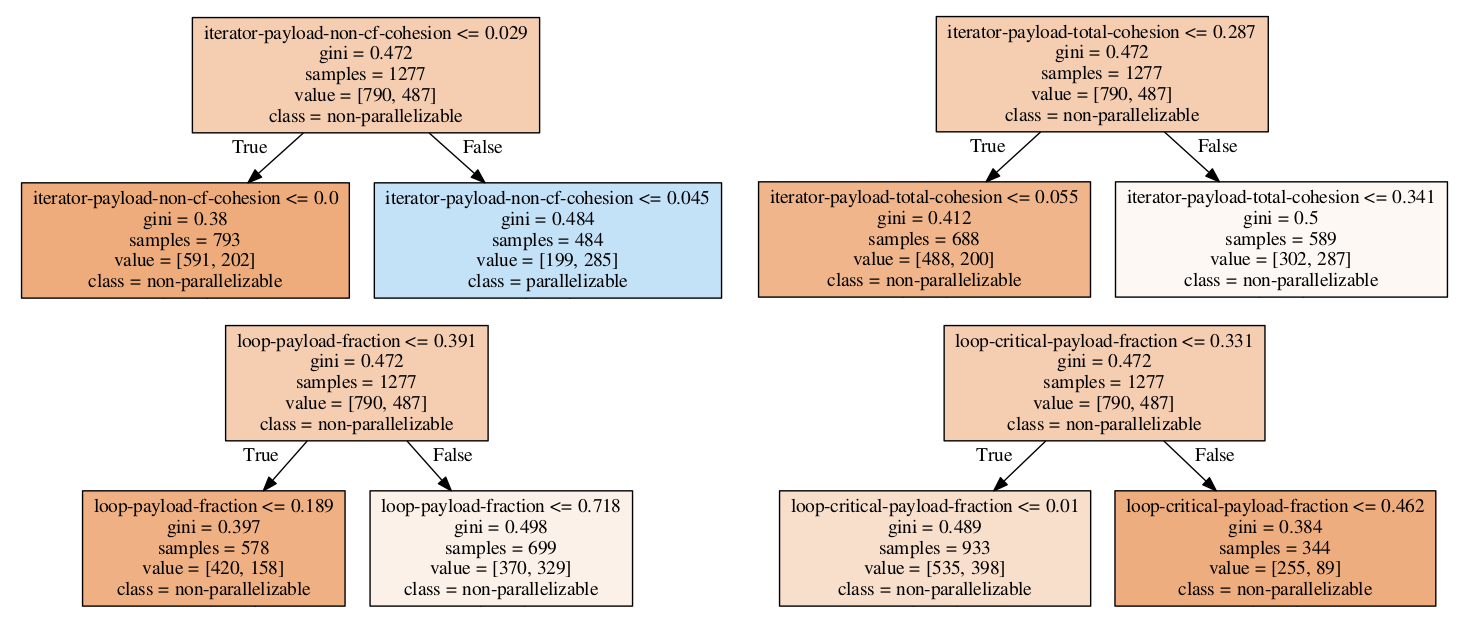
\includegraphics[width=\linewidth]{figs/decision-trees-single-metrics.png}
\caption{Decision boundaries and corresponding parallelizable/non-parallelizable probabilities for the best correlating single metrics.}
\label{decision-trees-single-metrics}
\end{figure}
\qquad We can see from the above figure \ref{decision-trees-single-metrics}, that if we use \textit{iterator-payload total cohesion} as a root node instead, we are going to get 0,287 decision boundary with 70\% non-parallelizible and 30\% parallelizible below 0,287 and 41\% non-parallelizible and 59\% parallelizible above the boundary. So, \textit{iterator-payload total cohesion} is slightly worse than \textit{iterator-payload non-cf cohesion}. It makes sence, since most iterators have control-flow structures, controlling conditions of the loop, but true dependencies are usually introduced by data edges from iterator to the payload. Metric \textit{loop critical payload fraction} can be used in the inverse way. If the value of this metric for a given loop happens to be greater than 0,33 decision boundary, then this loop is 74\% non-parallelizible. The latter result correlates with the common sense: the bigger critical payload part of the loop, the harder this loop is for dependence breaking and parallelization. The last metric in the figure \ref{decision-trees-single-metrics} is \textit{loop payload fraction}. We can see that the decision boundary for that metric is 0.391. So, if the payload of the loop happes to be less than 40\% of the total loop size, then this loop most likely is non-parallelizible with corresponding probability of approximately 73\%. That also makes sense, since big iterators include too much computations in them, which makes such loops hard to parallelize. Computations should be concentrated in the payload of the loop and iterators should be relatively simple.\newline
\null\qquad We don't necesserily need to use only single metrics. For a given loop we can compute a set of metrics and walk with their corresponding values down the decision tree in the figure \ref{decision-tree-depth-3}, which has been taught by parallelizible Intel C/C++ compiler. Use of multiple features increases the accuracy of results. For example, lets look at the figure \ref{decision-tree-depth-3}. Once we checked a loop being examing against the first root node rule and identified that the \textit{iterator-payload non-cf cohesion} metric happened to be greater than 0,03 decision boundary, we can check the second rule, namely $\textit{iterator-payload non-cf cohesion}\leq 0,21$. If we go along the blue (parallelizible) boxes, than we get $\frac{281}{434}\approx 65\%$ parallelizability chance against 59\% after only \textit{iterator-payload non-cf cohesion} boundary check. While parallelizability probabilities may not seem big enough for being worth the analysis, non-parallelizability probability in the left subtree can reach 85\% for a relatively big (374 samples) subset. For getting that estimate, metric values on a loop must satisfy to a system of 3 inequalities:\newline
\begin{equation*}
\begin{cases}
\begin{aligned}
\textit{iterator-payload non-cf cohesion}            &\le 0,029 \\[1ex]
\textit{loop payload fraction} &\ge 0.189 \\[1ex]
\textit{loop absolute size} &\leq 495
\end{aligned}
\end{cases}
\end{equation*}\newline
\null\qquad If we limit the depth of decision tree to 5 instead of 3, decision tree algorithm is going to add less parallelizability correlating metrics to consideration as well. Non-parallelizible predictions are not that interesting as parallelizable. Decision tree of depth 5 can predict parallelizability with better probabilities. For example, the two systems of inequalities below are going to conclude that a given loop is $\frac{207}{322}\approx 64\%$ and $\frac{56}{61}\approx 92\%$ parallelizable correspondingly.\newline
\null\qquad It would be of special interest to take a look at loops, which satisfy all these inequalitis, but nonetheless end up to be non-parallelizible. Such loops have not been parallelized by Intel ICC compiler, but have been classified as parallelizible by the set of metrics. If there are any among these loops, that are algorithmically parallel, but have not been parallelized by Intel compiler due to some lower-level technical issues, then these metrics find to be quite useful by telling software developed, that he should not listen to Intel compiler and take a closer human look at them. Section \ref{analysis-manual-analysis} conducts such an analysis.
\begin{equation*}
\begin{cases}
\begin{aligned}
\textit{iterator-payload non-cf cohesion}            &\ge 0,029 \\[1ex]
\textit{iterator-payload total cohesion} &\geq 0,21 \\[1ex]
\textit{loop critical payload fraction} &\leq 0,349 \\[1ex]
\textit{loop proper SCCs number} &\leq 1,5 \\[1ex]
\textit{critical payload true dependencies number} &\leq 6,5
\end{aligned}
\end{cases}
\end{equation*}\newline
\begin{equation*}
\begin{cases}
\begin{aligned}
\textit{iterator-payload non-cf cohesion}            &\le 0,029 \\[1ex]
\textit{iterator-payload total cohesion} &\leq 0,21 \\[1ex]
\textit{loop critical payload fraction} &\leq 0,349 \\[1ex]
\textit{loop proper SCCs number} &\leq 1,5 \\[1ex]
\textit{loop payload fraction} &\leq 0,575
\end{aligned}
\end{cases}
\end{equation*}\newline
    
\section{Manual analysis}
\label{analysis-manual-analysis}
\qquad Let's start from a trivial case and consider a loop, presented in listing \ref{lst:non-parallel-0}. This loop fills timer records array \textit{trecs[]} with timer reads. The latter are computed inside \textit{timer\_read()} function. Intel C/C++ compiler has to be conservative and does not parallelize that function, since it is not clear, whether there is a cross-iteration dependency introduced from inside the function, but the decision tree, presented in the figure \ref{decision-tree-depth-3} classifies that loop as parallelizible. Given that hint a programmer might check, if there are actually any states, preserved by \textit{timer\_read()} function from call to call, which might be distorted by the loop parallelization. This loop has \textit{iterator payload non-cf cohesion} equal to 0.0645, which correspond to parallelizible loops, according to results presented in the section \ref{analysis-single-metrics-vs-parallelizability}.              
\begin{lstlisting}[caption={Loop, which has not been parallelized by Intel C/C++ compiler, but does seem algorithmically parallelizible, given absense of cross-iteration dependencies introduced by the function call. }, captionpos=b, label=lst:non-parallel-0, float,floatplacement=H]
for (i = 1; i <= t_last; i++) {
	trecs[i] = timer_read(i);
}
\end{lstlisting}\newline
\null\qquad Another more elaborate case is presented in the listing \ref{lst:non-parallel-1}. Intel compiler failed to parallelize that loop nest, because it assumed that there is flow and anti dependencies between load from rhs[k][j][i][m] and store to rms[m]. But decision tree of depth 3 (see figure \ref{decision-tree-depth-3}) classifies that innermost loop as 65\% parallelizible and 35\% not, giving a programmer a little hope. Its classification could have been slightly better if there was not SCC inside the payload of the inner loop. Metric computing pass uses LLVM memory dependence analysis, which alike Intel compiler assumes dependencies between memory references to different arrays. Metric values for the innermost loop are: $\textit{iterator-payload non-cf cohesion}\approx 0.0357$, $\textit{iterator-payload total cohesion}\approx 0.3571$, $\textit{loop critical payload fraction}\approx 0.2963$.
\begin{lstlisting}[caption={\textit{SNU\_NAS/BT/src/error.c:84}. Loop, which has not been parallelized by Intel C/C++ compiler due to conservative anti and flow dependencies assumptions between references to rhs and rms. But these are different arrays and the loop actually computes reduction.}, captionpos=b, label=lst:non-parallel-1, float,floatplacement=H]
for (k = 1; k <= grid_points[2]-2; k++) {
	for (j = 1; j <= grid_points[1]-2; j++) {
		for (i = 1; i <= grid_points[0]-2; i++) {
			for (m = 0; m < 5; m++) {
				add = rhs[k][j][i][m];
				rms[m] = rms[m] + add*add;
			} 
		} 
	} 
}
\end{lstlisting}\newline
\null\qquad Assuming that a programmer accepted that metric hint, he decided to analyze and rewrite the loop with OpenMP pragmas (see figure \ref{lst:non-parallel-2}), since it it visible, that the loop computes reductions for all 5 rms array elements \ref{eq:equation-0}:\newline
\begin{equation}
rms\left[ m \right] = \sum\limits_{k \in grid\_points\left[ 2\right] -2}\sum\limits_{j \in grid\_points\left[ 1\right] -2}\sum\limits_{i \in grid\_points\left[ 0\right] -2} rhs\left[ k\right] \left[ j\right] \left[ i\right] \left[ m\right]
\label{eq:equation-0}
\end{equation}
\begin{lstlisting}[caption={Loop, which has not been parallelized by Intel C/C++ compiler, but does seem algorithmically parallelizible, given absense of cross-iteration dependencies introduced by the function call. }, captionpos=b, label=lst:non-parallel-2, float,floatplacement=H]
#pragma omp for nowait
for (k = 1; k <= grid_points[2]-2; k++) {
	for (j = 1; j <= grid_points[1]-2; j++) {
		for (i = 1; i <= grid_points[0]-2; i++) {
			for (m = 0; m < 5; m++) {
				add = rhs[k][j][i][m];
				rms_local[m] = rms_local[m] + add*add;
			} 
		} 
	} 
} 
for (m = 0; m < 5; m++) {
#pragma omp atomic
	rms[m] += rms_local[m];
}
\end{lstlisting}
\null\qquad Let's consider some more examples. Listing \ref{lst:non-parallel-3} shows another loop example, which computes reduction \ref{eq:equation-1}.
\begin{equation}
key\_buff\_ptr\left[ i \right] = \sum\limits_{j=0}^{i-1} key\_buff\_ptr\left[ i\right]
\label{eq:equation-1}
\end{equation}
\null\qquad It is clear, that the loop in listing \ref{lst:non-parallel-3} should be rewritten in order to be parallelizible, but Intel compiler gives just answer "no", but programmer takes a look at the values of metrics: \textit{iterator-payload-non-cf-cohesion}: 0.04, \textit{iterator-payload-total-cohesion}: 0.3, \textit{loop-critical-payload-fraction}: 0.3077. These values take the loop down the decision tree \ref{decision-tree-depth-3} into parallelizible classification. Programmer might take that hint and rewrite the loop.\newline
\begin{lstlisting}[caption={\textit{SNU\_NAS/IS/is.c:508}. Algorithmically parallelizible problem ends up hidden from compiler behind unsuccessful implementation.}, captionpos=b, label=lst:non-parallel-3, float, floatplacement=H, mathescape=true]
for( i=0; i<MAX_KEY-1; i++ ) {
	key_buff_ptr[i+1] += key_buff_ptr[i];
}
\end{lstlisting}
\null\qquad NAS benchmarks contain a lot of such examples. Listings \ref{lst:non-parallel-4}, \ref{lst:non-parallel-5} show some more of them.

\begin{lstlisting}[caption={\textit{SNU\_NAS/IS/is.c:468}. Algorithmically parallelizible problem ends up hidden from compiler behind unsuccessful implementation. Metrics: \textit{iterator-payload-non-cf-cohesion}: 0.0566, \textit{iterator-payload-total-cohesion}: 0.3208, \textit{loop-critical-payload-fraction}: 0.2143, \textit{loop-payload-fraction}: 0.6087}, captionpos=b, label=lst:non-parallel-4, float, floatplacement=H, mathescape=true]    
for( i=1; i< NUM_BUCKETS; i++ ) {  
	bucket_ptrs[i] = bucket_ptrs[i-1] + bucket_size[i-1];
}
\end{lstlisting}

\begin{lstlisting}[caption={\textit{SNU\_NAS/LU/src/l2norm.c:57}. Intel compiler refuses to parallelize that reduction problem due to assumed true and anti dependencies between memory references to different sum and v arrays. Inner loop metrics: \textit{iterator-payload-non-cf-cohesion}: 0.0331, \textit{iterator-payload-total-cohesion}: 0.3967, \textit{loop-critical-payload-fraction}: 0.1364, \textit{loop-payload-fraction}: 0.8148}, captionpos=b, label=lst:non-parallel-5, float, floatplacement=H, mathescape=true] 
for (k = 1; k < nz0-1; k++) {
	for (j = jst; j < jend; j++) {
		for (i = ist; i < iend; i++) {
			for (m = 0; m < 5; m++) {
				sum[m] = sum[m] + 
					v[k][j][i][m] * v[k][j][i][m];
			}
		}
	}
}
\end{lstlisting}

\section{Statistical analysis}
\label{analysis-statistical-analysis}
\qquad Statistical learning techniques can be used to compare relative performance of software source code metrics in the task of parallelizability classification. This section views loop parallelizability as a machine learning problem. Metrics represent features of loops. Intel C/C++ compiler gives an expert-opinion and labels (classifies) loops as parallelizible or not. Three ML algorithms have been applied to the dataset presented in figure \ref{analysis-data-table}: Support Vector Machines (SVM), decision tree classifier, neural network based Multi-layer Perceptron (MLP). All machine learning metric set studies have been conducted with the help of pandas \cite{python-lib-pandas} and scikit-learn \cite{python-lib-scikit-learn} python packages. Detailed description of all algorithms, techniques and all underlying mathematical foundations can be found in the introduction to statistical analysis book \cite{statistical-learning-book}.\newline
\null\qquad Table \ref{single-metric-ml-table-0} below presents results obtained for every single loop parallelizability metric out of proposed metric set (see section \ref{metrics-metric-groups}).
\begin{sidewaysfigure}[htb]
\centering
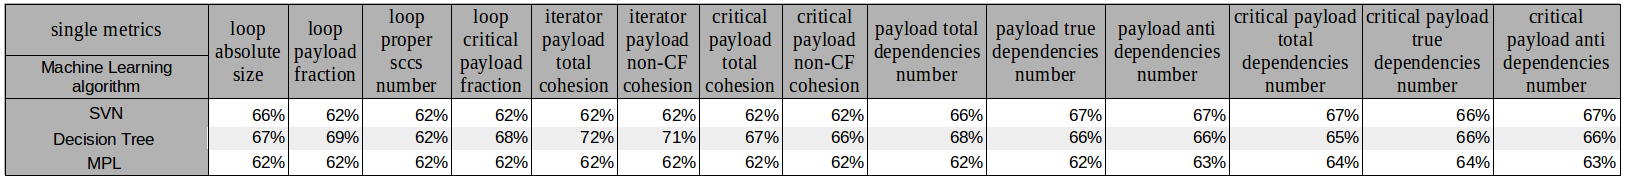
\includegraphics[width=\linewidth]{figs/single-metric-ml-table-0.png}
\caption{Average accuracies of parallelizability predictors. Each predictor has been trained with only one feature (table columns). Different machine learning techniques (SVN, Decision Tree, MPL) have been used for training. Percentages in the table represent mean prediction accuracies. K-fold (K=15) cross validation technique has been used to partition samples from \ref{analysis-data-table} into training and testing sets. Different K numbers (5, 10, 20, 30) produce approximately the same mean accuracies (see figure \ref{single-metric-ml-table-1}) for the full set of K values.}
\label{metric-set-ml-table-0}
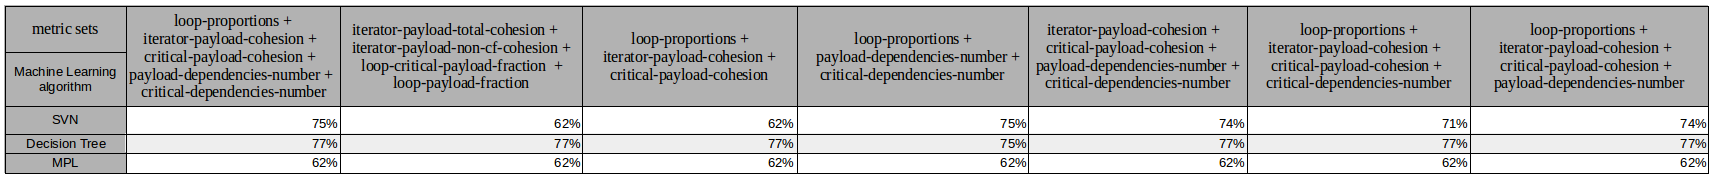
\includegraphics[width=\linewidth]{figs/metric-set-ml-table-0.png}
\caption{Average accuracies of parallelizability predictors. Each predictor has been trained with sets of metrics. Results are presented in the same form as in table \ref{single-metric-ml-table-0} above. Full table, with all K values (5,10,15,20,30) is available in the figure \ref{metric-set-ml-table-1} of the appendix.}
\label{single-metric-ml-table-0}
\end{sidewaysfigure}\newline 
\null\qquad Every single metric has been used as a loop feature, to train different machine learning models to classify loops as parallelizible or not. Above table \ref{single-metric-ml-table-0} reports on accuracies of corresponding trained predictor models. In order to train every single model, the dataset \ref{analysis-data-table} has been partitioned into training and testing subsets. Partitioning has been done with K-fold method. This method splits all data samples into K equal subsets. Then it chooses one of these spilts as a testing set and uses all the rest as a training set. This process is repeated K times to cover all possible cases. Then K-fold partitioning might be applied again, but with different partitions. That application might be repeated N times. For the table \ref{single-metric-ml-table-0} above K=15, N=5. For every training and testing run predictors report accuracy. All these accuracies have been averaged to just one percentage, presented in the table \ref{single-metric-ml-table-0} above.\newline
\null\qquad Exactly the same experiment (with K=15 and N=5) has been conducted with different sets of metrics used as features of predictor models. Table \ref{metric-set-ml-table-0} below shows collected results.
\null\qquad Results, presented in tables \ref{single-metric-ml-table-0} and \ref{metric-set-ml-table-0} do not change significantly with K and N variations. Corresponding tables \ref{single-metric-ml-table-1} and \ref{metric-set-ml-table-1} in the appendix show the whole sets of accuracies for K equal to 5, 10, 15, 20 and 30.\newline
\null\qquad It is visible from the tables, that decision tree learning method works the best in both cases: for models with single loop metrics as featues, as well as for models with sets of metrics as features. For models with single metrics as features, decision tree makes predictions with accuracy around 65-70\%, with 71-72\% for two \textit{iterator payload cohesion} metrics. These metrics seem to work a bit better than others, what corerlates with conclusions made in section \ref{analysis-single-metrics-vs-parallelizability} of this chapter.\newline
\null\qquad When we use sets of metrics as machine learning model features, accuracies these machine learning predictors can achieve are a bit higher. Decision tree based algorithm can achieve accuracy of 77\%. This learning algorithm works comparably for all sets. For the set in the first column of table \ref{metric-set-ml-table-0} (with all 13 metrics out of 5 groups used as features) decision tree works as good as for the set in the second column (just 4 most parallelizability correlating metrics). On the other hand, accuracies of SVN based model tend to be noticably higher for models with more metrics as features. Table \ref{metric-set-ml-table-0} shows, that when we add dependencies number metrics to feature sets we get increaced prediction accuracy. It might look weird in the light of absence of any correlations between dependencies number metrics and loop parallelizability, as was shown in the section \ref{analysis-single-metrics-vs-parallelizability}. \textit{Loop proportion} metrics combined with \textit{loop cohision} metrics tend to work much worse, than \textit{loop proportion} metrics combined with \textit{loop dependencies} number metrics. This result is also a bit surprising, because \textit{loop cohesion} metrics correlate with parallelizability better, that \textit{loop dependencies number} metrics.\newline
\null\qquad Results of decision tree learning algorithm corelate better with the results presented in section \ref{analysis-single-metrics-vs-parallelizability} of this chapter, than SVN results. MPL accuracies do not seem to change with different feature sets at all.  
          
\chapter{Results}
\label{results}
\qquad This chapter summarizes the main results of the undertaken MSc by Research 2018 project and describes its workflow as it happened. In short, the main results of the undertaken MSc by Research project can be described with several points:
\begin{enumerate}[align=left,leftmargin=*]
\item \textbf{Software source code parallelizability metrics search has been conducted. MSc bt Research project has been set up.}\newline
\null\qquad A body of literature has been searched through in an attempt to find any software source code metrics, applicable to the software parallelizability problem. While there are a lot of metrics aimed at judging about software quality (maintainability, readability, etc.), none were proposed to judge about software parallelizability. The only metrics in the subfield of parallel computation represent different variations of program execution time speedup ratio. Short report is given in the sections \ref{background-software-metrics-in-cs} and \ref{background-metrics-parallel-computing} of the background chapter \ref{backgroud}.\newline
\null\qquad It was decided, that Program Dependence Graph (PDG) (proposed in the paper \cite{pdg-paper}) is going to be an intermediate program representation, parallelizability metrics would be computed on. Moreover, parallelizability metrics would use loop decoupling and loop iterator recognition results (proposed in the paper \cite{iterator-recognition-paper}) as a prerequisite for their further computation. The first metric to be computed was decided to be \textit{loop payload fraction} (see \ref{metrics-loop-payload-fraction}). LLVM compiler components library \cite{llvm-official-website},\cite{llvm-paper} was chosen for the MSc project to be based on.	
\item \textbf{Development of LLVM-based metric computing tool.}\newline 
\null\qquad This stage took the most of the time and efforts. As a result PPar tool (described in \ref{ppar-tool} and hosted on the GitHub \cite{ppar-tool}) ($\approx$ 4750 C/C++ lines of code) has been developed. The tool development started straight after the first metric ideas were conceived (end of January 2018).\newline
\null\qquad The PDG intermediate representation and all algorithms, proposed and described in \cite{pdg-paper} and \cite{iterator-recognition-paper} have been implemented from the scratch. This took a significant project start-up overheads. Development of dependence graph intermediate representation on top of LLVM IR along with loop decoupling and iterator recognition algorithms (strongly connected components search) took more than a month of time. During that period LLVM DEBUG() prints served as the only debugging and validation means.\newline
\null\qquad After the first graph visualization facilities (thanks to Graphviz and DOT) had been added the project, the first research work has actually started. Along with further validation, debugging and development of the tool, first metrics started to appear on the small hand-written tests. Metric values have been manually validated against PDG and its SCCs DOT graph visualizations. Visualizations of these PDG and their SCCs served as an inspiration for the proposal of a new metrics.\newline
\null\qquad By June 2018, 17 metrics have been devised and integrated into the developed PPar tool framework. Metric values could be obtained on the small set of hand-written tests. These values have been manually verified with graph visualizations. This work has been reported during the Intermediate Progress Review held on the 7$^{th}$ of June 2018.                    
\item \textbf{Devised metric values have been collected on the NAS benchmark suite.}
	
\item \textbf{Analysis of devised parallelizability metrics.} Once all metric values had been gathered for all NAS benchmark loops and all loops had been classified with Intel C/C++ compiler, the final stage of the project could be started.     
	
\end{enumerate}





\qquad The overall picture in the matter of software source code (loops in particular) metrics for  parallelisability resembeles that of the software quality metrics. Software quality (say, maintenance) is a complex notion. To judge about good or bad software design one must posses vast software engeeniring expertise and skills. Metrics like cyclomatic complexity can be used as supplementary to manual analysis, but the values they give must be examined by a human with a deep understanding of the software quality question. Although, their values might sometimes correlate with the understanding of a sound software design, these metrics should not be applied blindly.\newline
\null\qquad Software parallellizability property is not a simplier one. Despite the fact, that all examined metrics have grounds to be proposed and are not randomly selected, their parallelizability correlations are limited and there are always special cases, which break generally established rules and patterns.\newline


\null\qquad However, the working framework, developed withing that  MSc by research project, is ready and can be used for further metrics research and analysis. It is quite easy to add new metrics to the tool. Tool provides visualization facilities for dependence graphs and loop iterator/payload decomposition. New metrics might be added. Alternatively, existing metrics might be fine-tuned as well. This work might be the one on the relatively new direction. Application of machine learning in compilers. Since all machine learning methods require some quantitative features, these loop metrics might be an attempt in their establishment. Modern compilers apply a set of optimizations: loop unrolling, peeling, splitting. Correlations between these metrics and these properties (like loop unrollability) might be examined towards development of machine-learning driven compiler optimizers.\newline
\null\qquad A lot of time has been spent on the development of the tool itself and the first, suitable for analysis, results appeared quite late in the timeframe of the project.         
\chapter{Future work and current limitations}
\label{future-work}
\qquad The major inherent problem of the done MSc research work, is that under given timeframe it was decided to use Intel C/C++ compiler as a parallelizability expert. While ICC is pretty good in program parallelization, there are still cases, where it does not parallelize loops, which could be parallelized. If there was an ideal parallelizing expert available, then some of the red dots in the presented figures would be green, which could slightly change the results. Seoul National University implementation of NAS benchmarks has two versions of the benchmarks: sequential, and the one with added OpenMP pragmas. Ideally, these pragmas could be used as answers to the parallelizability question. It was just technically easier to use ICC compiler to get the answers.\newline  
\null\qquad While there were some little correlations between proposed metrics in their current form and loop parallelizability property, it is clear, that in order to get ideally expected correlation results (if it is principally possible to achieve it with certain precision), these metrics must be tuned, refined and probably supplemented with additional ones. In the current project state it is going to be a way easier. Working research framework has been developed in the form of PPar tool (see \ref{ppar-tool}) and surrounding scripts. All the work from C/C++ source code at the input of LLVM to the final metric figures of Python machine learning scripts has been done. PPar tool is designed in such a way, that it can be easily extended with new metrics without much efforts. Graph visualization facilities can be used to study and refine currently proposed set of metrics.\newline
\null\qquad It is possible to look at the done work from another more general angle. Computation of different numeric features lies at the basis of any machine learning technique. Some loop features have been computed in this work. These features have been examined (withing certain limits) against loop parallelizability property. The same features can be examined against different loop properties, like applicability of different loop optimizations. This work might lie on the path towards machine learning driven optimizing compilers. Apart from loops, some numeric features can be computed for different objects like program data structures, which can enable their identification by compiler.
%% ... etc ...

%%%%%%%%
%% Any appendices should go here. The appendix files should look just like the
%% chapter files.
\appendix
\chapter{Appendix}
\label{appendix}

\qquad The same dataset has been also projected onto 2D plane, as illustrated in the figure \ref{metrics-pca-13-to-2}.

\begin{figure}[htb]
	\centering
	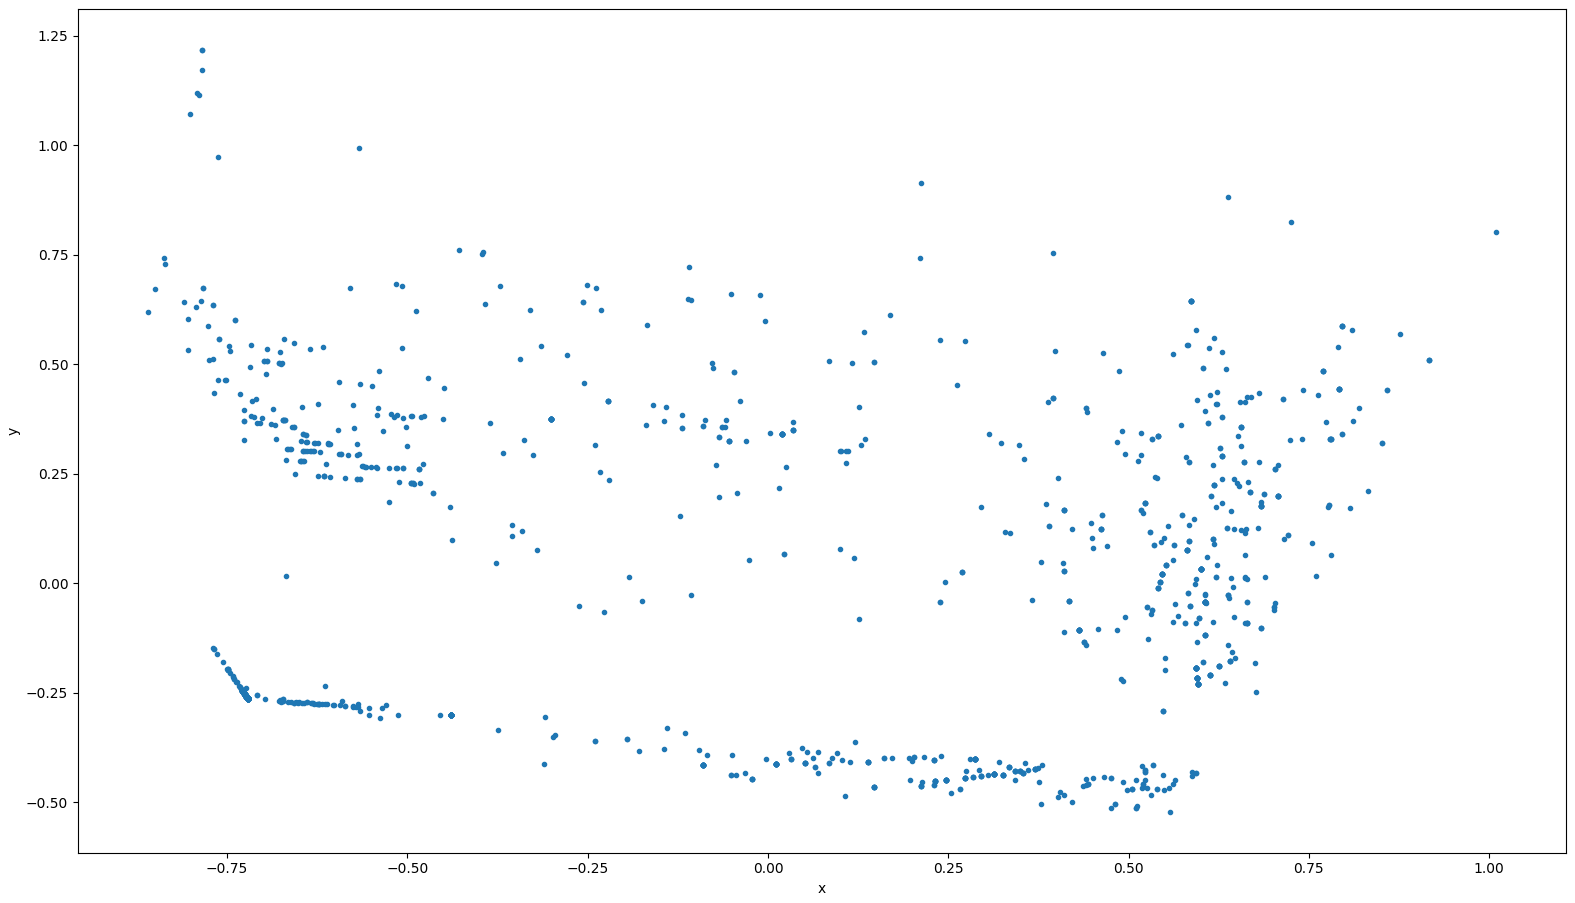
\includegraphics[width=\linewidth]{figs/metrics-pca-13-to-2.png}
	\caption{Visualisation of loop metrics dataset (13-dimensional metric vectors have been projected onto 2d space thanks to PCA algorithm) - blue dots correspond to metric values on single loops.}
	\label{metrics-pca-13-to-2}
\end{figure}

%% ... etc...

%% Choose your favourite bibliography style here.
%%\bibliographystyle{plain}
\bibliographystyle{unsrt}

%% If you want the bibliography single-spaced (which is allowed), uncomment
%% the next line.
% \singlespace

%% Specify the bibliography file. Default is thesis.bib.
\bibliography{bibliography}

%% ... that's all, folks!
\end{document}
